\subsection{ESP32 Firmware Code[YJ]}

The following sections below will provide the reader with knowledge of Firmware code.
By doing so, the reader will understand how all the pieces of software fit together and the intensive testing done to test the features.
Throughout this section, the reader will learn how the raw sensor values received help produce meaningful behavior on the product side.
I will discuss the knowledge and skills I gained during this process.

The hardware controller chosen for this project was from the ESP-32 family.
The system was architected to have its operating system using FreeRTOS.
The system uses software timers to calculate how long the door has been kept open.
The calibrated sensor values, the door and alarm states are packaged as a JSON document and transmitted to the Raspberry Pi through serial communication.
The code development and integration started after proof that the individual sensors would behave and operate as designed during our initial testing.
The tasks and timers created matched the design specification that was agreed upon by the group.

Attached below is the system-level diagram for the microcontroller.
The weight values are stored and used as a comparison again for the next reading to determine the object's direction.

\begin{figure}[H]        
    \centering
    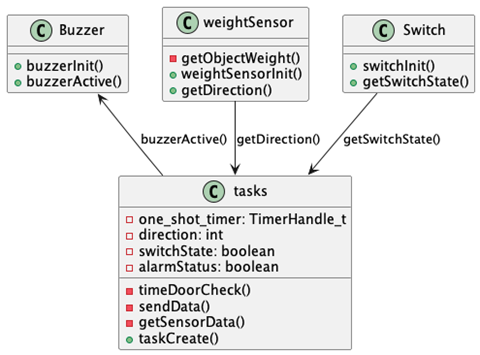
\includegraphics[width=.66\textwidth]{Chapter 4/Firmware Code ESP32/ESP32ClassDiagram.png}
    \caption{UML for System Machine}
\end{figure} 

\subsubsection{RTOS [YJ]}

RTOS is commonly known as Real Time Operating System.
It is an operating system with key features such as predictability and determinism.
An operating system is a computer program that supports a computer's fundamental functions and provides services to other programs that run on the computer.
RTOS creates tasks based on priority while keeping the context switching to the minimum.
Context switching is storing the current state of the thread that is resumed later at a different point in time.
It allows multiple processes to share the same CPU, which is the core feature of multitasking operations.
\cite{RTOS:1} \cite{RTOS:2}

The RTOS kernel used in this project is FreeRTOS.
FreeRTOS is small and light to run on small microcontrollers.
It is preferable because most microcontrollers do not have enough RAM and flash storage.
FreeRTOS also makes it easy to connect IoT( Internet Of Things) devices to the AWS( Amazon Web Services )services by Amazon.

Espressif Systems is a privately held fabless semiconductor company.
They provide wireless communications and Wi-Fi chips in mobile devices and the Internet of Things applications.
The Smart-Fridge uses the ESP-32-Wroom-32 microcontroller.
The Software Development Kit provided by Espressif has a different version of FreeRTOS with slight variations from the vanilla FreeRTOS natively used.
It allows us to freely call the API functions of the FreeRTOS without having to download or include any library.

For this project, to keep in mind simplicity and rapid prototyping and testing requirements, I have designed the tasks system as follows.

The threads generated using "xTaskCreate" are getSensorData and sendData.
The data shared between these two tasks is handled through a message queue buffer.
It prevents memory corruption where one thread reads while the other writes simultaneously.
This message queue is made by "xQueueCreate".
The data collected in the "getSensorData" task is sent to the message queue by "xQueueSend", and the "sendData" receives the latest data on this message stack by “xQueueReceive".

I initially struggled to get the tasks to run on the microcontroller as I was dealing with dangerous memory access errors.
After reading the documentation provided on the FreeRTOS website, I was able to debug the solution and solve the issue.
To understand the timing difference and priority between the two threads, I wanted to provide the lowest delay possible for the sensors so that the system would not miss any event that occurred.
The delay on the data transfer is at 1 second.
It gives time for the processor to average the raw readings and provides accurate results.

\subsubsection{Software Timer [YJ]}

A software timer is a function that executes after a pre-defined period.
The task called after the timer should perform simple short tasks such as toggling a state or changing a variable so that the system does not hang in this state or accidentally trigger the watchdog and reset the microcontroller.
The function executed by the timer is called the timer's callback function.

As the name suggests, the software timer calculates the time by the operating system and does not rely on the hardware.
The advantages of the software timer are that they do not add any processing overhead and take up minimal space on the applications binary.

In our application, we first declare the software timer and define its duration along with if it is a timer to be repeated automatically by the system or manually triggered by a set condition.
The Timer callback function changes the state of the "alarmState", which activates the buzzer till the door of the fridge is closed.

\subsubsection{ESP-Pi Communication [YJ]}

The ESP-Firmware must communicate with the Raspberry Pi.
The messages to the pi are on an agreed-upon pre-defined data table mentioned below.
The table mentioned below tells the Pi the current state of the fridge regarding the alarm, door and objects entering and leaving the fridge.

% Please add the following required packages to your document preamble:
% \usepackage{longtable}
% Note: It may be necessary to compile the document several times to get a multi-page table to line up properly
\begin{longtable}[c]{|l|l|l|l|}
    \caption{ESP to PI Comms}
    \label{tab:yohan}\\
    \hline
    Number &
      Message &
      Value &
      Purpose \\ \hline
    \endfirsthead
    %
    \endhead
    %
    1 &
      DIRECTION\_NO\_CHANGE &
      0 &
      \begin{tabular}[c]{@{}l@{}}Object weight leaving and\\ entering the fridge is the same\end{tabular} \\ \hline
    2 &
      DIRECTION\_LEAVE\_FRIDGE &
      1 &
      \begin{tabular}[c]{@{}l@{}}Object left the fridge as weight\\ drops to 0\end{tabular} \\ \hline
    3 &
      \begin{tabular}[c]{@{}l@{}}DIRECTION\\ \_ENTER\_FRIDGE\end{tabular} &
      2 &
      \begin{tabular}[c]{@{}l@{}}New Object enters the fridge\\ as weight is different to\\ previous object\end{tabular} \\ \hline
    4 &
      DOOR\_OPEN &
      1 &
      \begin{tabular}[c]{@{}l@{}}HAL sensor returns HIGH state\\ hence door is open\end{tabular} \\ \hline
    5 &
      DOOR\_CLOSE &
      0 &
      \begin{tabular}[c]{@{}l@{}}HAL sensor returns LOW as\\ magnet is in contact with the\\ sensor hence door is closed\end{tabular} \\ \hline
    6 &
      ALARM\_ACTIVE &
      1 &
      \begin{tabular}[c]{@{}l@{}}Door kept open longer than\\ predefined safe limit hence\\ ALARM is activated\end{tabular} \\ \hline
    7 &
      ALARM\_INACTIVE &
      0 &
      \begin{tabular}[c]{@{}l@{}}Door kept open longer than\\ predefined safe limit hence ALARM\\ is activated\end{tabular} \\ \hline
    \end{longtable}

Three states tell the direction of the object, they are no changes in the path, an item is leaving the fridge, and an item is entering the smart fridge.
The other values are booleans that tell the Pi if the door is open and if the alarm has been raised for the door being open for too long.

Communication between the ESP32 and the Pi happens through the UART protocol.
A JSON packet is packaged with the three states, as seen below and sent to the Pi.
JSON serialisation is favourable to transferring data as the system can send all the information in a single message packet.
The drawback of this system is that there is only one-way communication between the two boards using one UART serial port.

The fix is to utilise the second set of UART pins on the Esp32 if the ports are unused.

The ArduinoJSON library determined how the messages were packed on a JSON document and sent via the serial port.
The JSOC document requires a key that maps to a value.
I struggled with sending the JSON document through the second UART port on the development board.
The board's documentation sheet mentioned that there were two sets of UART pins enabled on the development board but only able to transmit and receive.
I tested this by connecting the pins to an Arduino UNO board running a deserialisation script that printed NULL but printed the values using the default pins for Transmit and receives on the ESP-32 board.

\begin{figure}[H]        
    \centering
    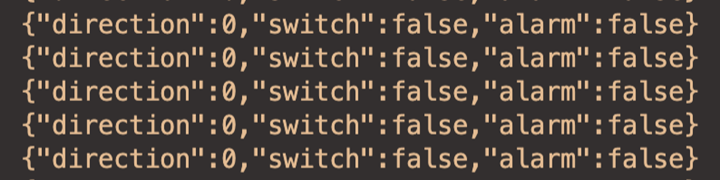
\includegraphics[width=1\textwidth]{Chapter 4/EspToPiCommunication/JSONPACKET.png}
    \caption{JSON Packet Sample}
\end{figure} 

\begin{figure}[H]
    \begin{subfigure}{.5\textwidth}
      \centering
      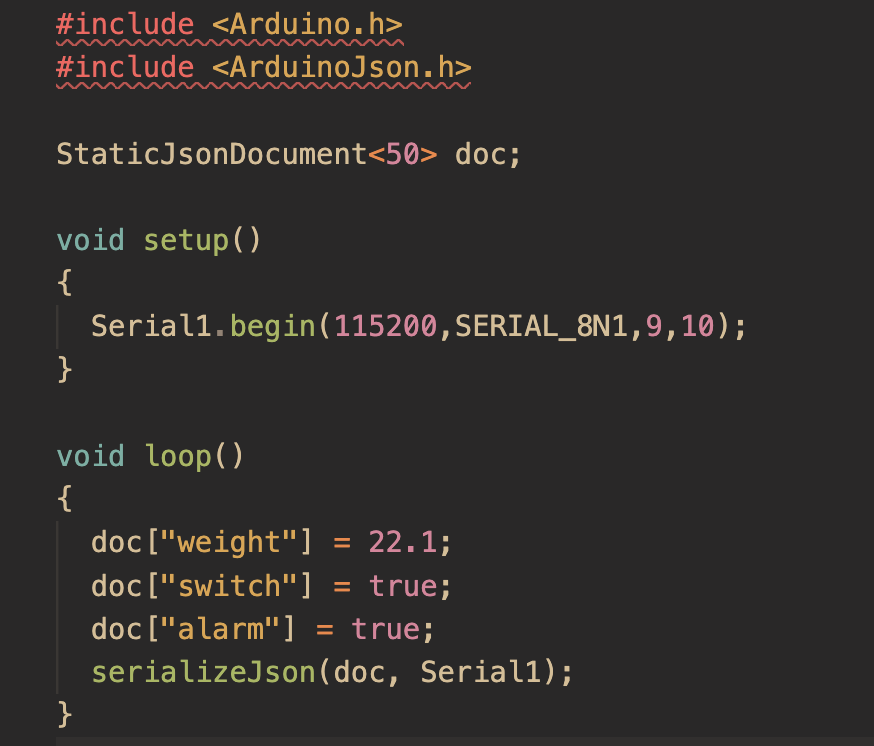
\includegraphics[width=.66\linewidth]{Chapter 4/EspToPiCommunication/serial.png}
    \end{subfigure}%
    \begin{subfigure}{.5\textwidth}
      \centering
      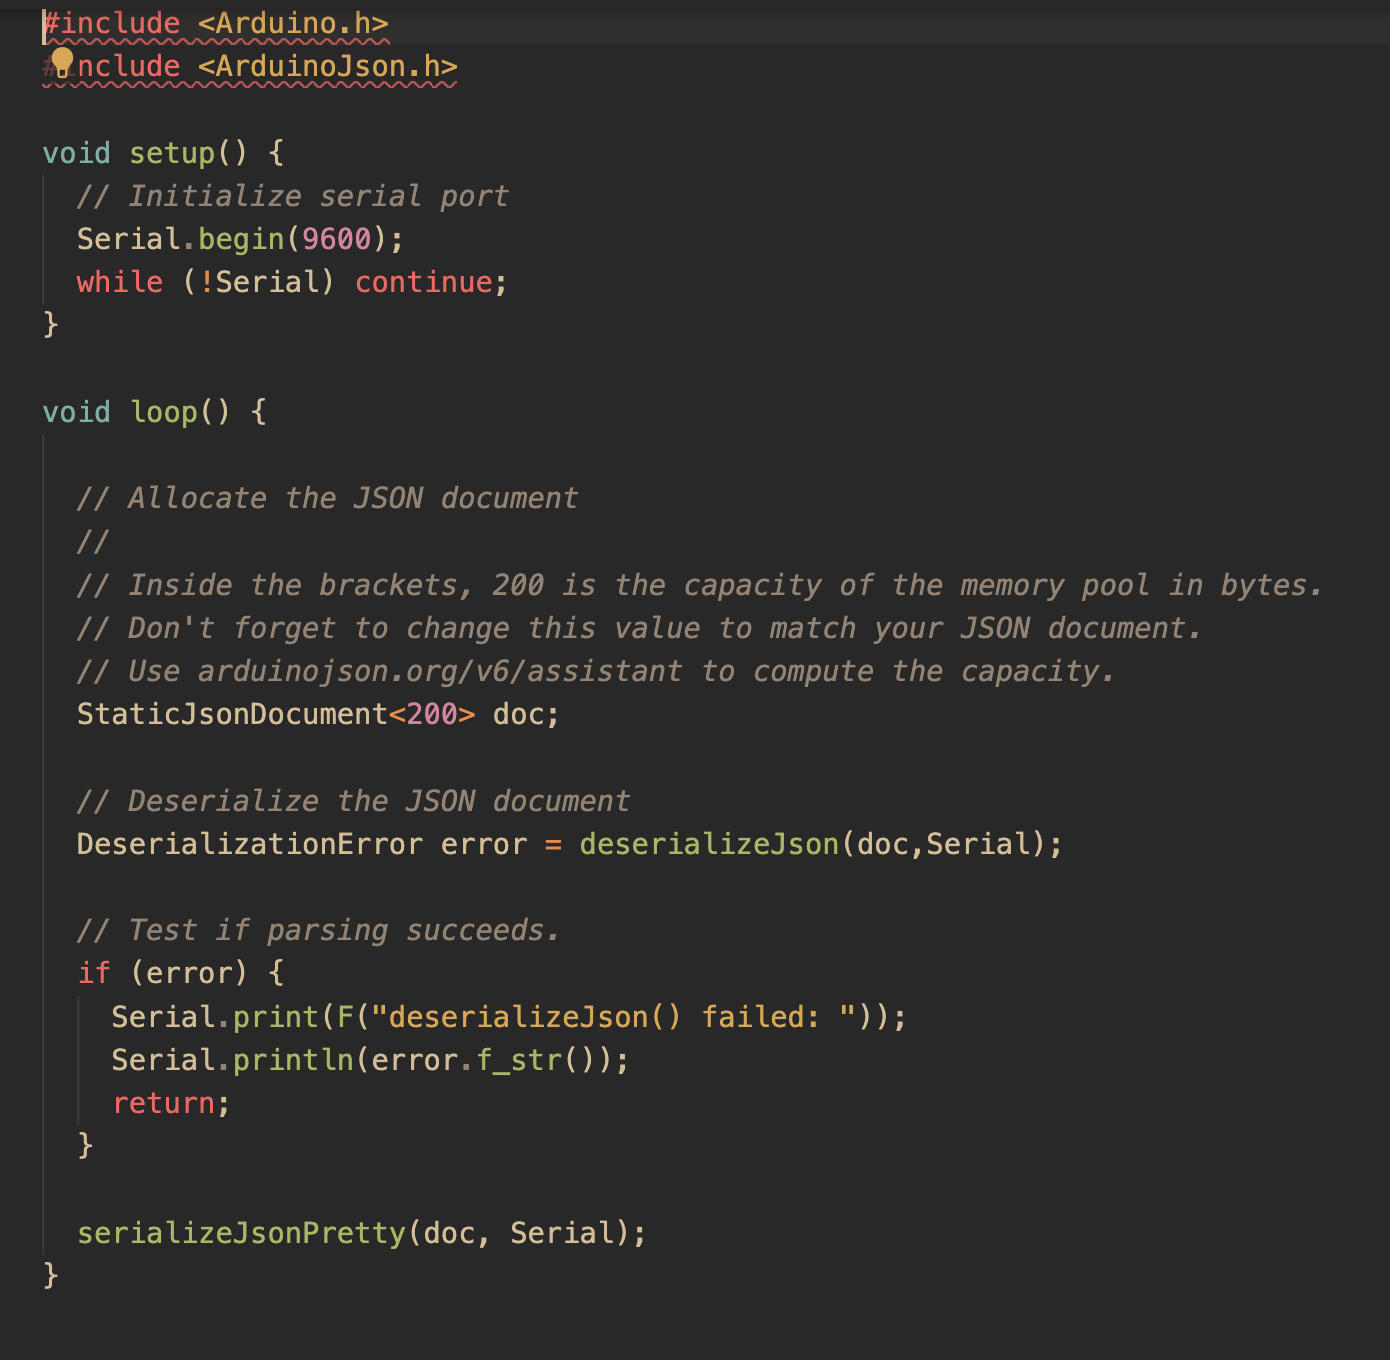
\includegraphics[width=.66\linewidth]{Chapter 4/EspToPiCommunication/deserial.png}
    \end{subfigure}
    \caption{Serialisation and Deserialisation Scripts}
\end{figure}

\subsection{Raspberry Pi Overview [AW]}

As mentioned in the system overview, the Raspberry Pi receives a JSON packet from the ESP-32 which will alter the response of the Pi and change the data to be sent to the database.
The JSON itself is discussed at further length in the Pi Serial Input section.
The Raspberry Pi also handles the camera, the computer vision calculations, and the networking to the database.
These are the features that will be explored in this section, starting with the different computer vision methods utilized.

\subsubsection{Pi Object and character recognition [IB]}

There are two tasks that utilize object and character recognition.
The first one is the expiration date which is implemented using a OpenCV and a python library and the output gives the characters, in this case the numbers of the expiration date.
The second task is to take an image of the product and using an already trained model, the product will be classified and return its class.
	

\subsubsection{Expiration Date - Character Recognition [IP]}

The implementation of the expiration date recognition requires loading an image and then processing it to be able to use a function that will extract the digits detected.
The function that identifies and extracts the characters comes from a library called PyTesseract.
PyTesseract is a python tool used for optical character recognition, that recognizes and extracts characters on an image \cite{pypiPytesseract}.
The code written can be found in a repository on github.
In the code implemented, the image is loaded using the OpenCV library's image read function (imread) and then converted from BGR to RGB channel ordering, again using an OpenCV library function.
The function named image\_to\_string from PyTesseract tool is then called which takes in the rgb image and stored in a variable.
The variable holds the text of the characters extracted and is the output of the code.

A virtual environment was used to run the code in which the PyTesseract was installed, as well as the rest of the necessary libraries such as OpenCV.

The PyTesseract tool is an engine that functions by following a series of stages that include finding and nesting the outlines, organising into text lines, and then the recognition follows using an adaptive classifier.
The first step is inspecting the nesting of the general outlines as well as the smaller ones.
The outlines are assembled into objects which are then organised into text lines.
The next step includes testing whether the test lines are fixed pitch, and the text lines are divided into words according to the spacing between them.
Recognition of the text is the next process that takes place, which is done by firstly recognising each word and then passing it into a classifier.
The process is repeated for the case where the classification didn't successfully recognize words \cite{TesseractOverview}.

The performance of the expiration date detection was tested using images initially with just numbers and then of more complicated images, meaning the products with expiration date on them.
In the images with just numbers taken from google, the average performance was satisfactory as the output of the code returned the number that was embedded on the image.
The images that contained the products had a poorer performance as the majority of the images were not as clear regarding the intensity of the image and the shape of the characters.
Initially, this was a major drawback as other than the images used for testing from the internet, images were captured from the ESP32 camera but failed the tests, as they were very blurry and unfocused.
This was discussed with the rest of team, and it was decided that the ESP32 camera wouldn't be used, and a web camera would replace it.
Images captured from the webcam were then tested and had a much-improved performance.
The lighting when the image is captured is highly important as it can zero the possibility of the function's ability to read and extract the characters.

\subsubsection{Product detection – Object recognition [IP]}

The product detection was implemented by training a convolutional neural network using a public dataset.
The dataset included images of grocery items of 43 different classes, that included mainly vegetables and fruits, as well as other products.
There are a total of 5,571 images that are used for training, testing and validation sets.
The model is trained on this dataset, and then the image captured from the fridge is tested on the model.

\subsubsection{Background theory on design implementation [IP]}

A convolutional neural network (CNN) was used as it is considered as one of the most efficient algorithms for image classification.
In this case, a simple architecture of a CNN was designed with the addition of using a pre-trained model, using transfer learning.
A model consists of layers in which the training of the data takes place.
The first layers of a model train the data on more generic features such as shapes, edges, and colours, whereas the higher layers learn more complex and specific features.
A more efficient way to train the data would be to use a model that has been pre-trained in the more generic task features and complete training only for the more complex task features.
The pre-trained model used is the VGG16 architecture which consists of 16 layers that hold the learnable parameters (weights), 3 convolutional layers, 5 max pooling layers and 3 dense layers, in total 21 layers \cite{VGG16overview}.
The convolutional layers use filters, or kernels with the purpose of performing the convolution operation on the input and give an output of a feature map that comprises the features detected.
The max pooling layers perform an operation that takes the maximum value of a specified region on the feature map with the aim to reduce its dimension.
Lastly, the dense layers contain the neurons that are connected to the ones in the previous convolutional layers with the aim to perform the classification.
The architecture of the VGG16 architecture is shown in figure \ref{fig:cnn}.

\begin{figure}[H]        
    \centering
    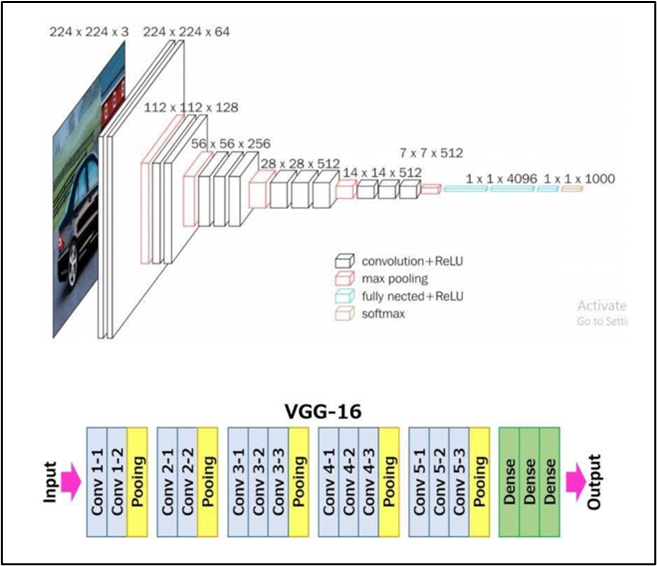
\includegraphics[width=.66\textwidth]{Chapter 4/CNN/VGG-16.png}
    \caption{VGG16 Architecture \cite{VGG16overview}}
    \label{fig:cnn}
\end{figure} 

\subsubsection{Pre-processing of the dataset [IP]}

The dataset that is used as the input to train the model required processing into the appropriate train, test, and validation sets.
The training and validation sets contain the data based on which the model is trained on, and the test set contains the data used to test the performance of the trained model.

The dataset consists of 3 main categories, which were vegetables, fruits, and packages.
Within each of these three categories, there were subcategories which resulted in 43 classes in total from all categories.
The goal of the classifier is to classify what the product is, so between these 43 classes, and not to which generic group/category they belong to.
Therefore, the 3 categories were removed, and all 43 classes were put under the same folder, for all three training, testing and validation sets.
The dataset had already completed the splitting between the sets.
The dataset was taken from a repository \cite{dataset} and was used for a research paper.

\subsubsection{Model architecture [IP]}

For the model architecture, as mentioned before in the background theory, a VGG16 pre-trained model was used for which the features learned were stored in some filed, known as the bottleneck files.
The bottleneck files were created for all three tests (training, testing and validation) and were loaded to be used as the according data.
The labels for each class were generated using the ImageDataGenerator, a TensorFlow pre-processing function and were transform the data to a binary class matrix before passing it to the model.
After the data and the labels for each set were prepared, the model architecture was designed.
A sequential model was initialised, as the following layers used are in a linear stack.
The first layer, which is a Flatten layer, contains the data that has been taken from the bottleneck files.
The dense layers contained the activation function that determined the values that the neurons would hold.
The dropout layers randomly neutralise some neurons during the training with the aim of preventing overfitting, meaning the model not being able to generalise and only being able to accurately predict the already trained data.
A SoftMax activation function was used to compute the probabilities for the output for all the classes.
After the model's architecture design, the data was fitted in the model and the training occurred.
A batch size and number of epochs was specified.
After the training, the weights of the model were saved, and an accuracy and loss score were printed.


\subsubsection{Expiration Date Evaluation [IP]}
The performance of the expiration date detection was tested using images initially with just numbers and then of more complicated images, meaning the products with expiration date on them.
In the images with just numbers taken from google, the average performance was satisfactory as the output of the code returned the number that was embedded on the image.
The images that contained the products had a poorer performance as the majority of the images were not as clear regarding the intensity of the image and the shape of the characters.
Initially, this was a major drawback as other than the images used for testing from the internet, images were captured from the ESP32 camera but failed the tests, as they were very blurry and unfocused.
This was discussed with the rest of team, and itH was decided that the ESP32 camera wouldn't be used, and a web camera would replace it.
Images captured from the webcam were then tested and had a much-improved performance.
The lighting when the image is captured is highly important as it can zero the possibility of the function's ability to read and extract the characters.

\subsubsection{Product Detection Evaluation [IP]}
For the testing part of the product detection, two functions were created, one to read the image and another to predict the class of the image based on the model.
The first function that reads the image, converts it to an array of values and normalises by dividing values by 255 for the computation to be faster.
The second function loads the trained model and weights and stores them in a variable named reconModel, for reconstructed model.
After all the possible classes are defined, the image reading function is called and then the image is used to perform the prediction.
After testing the model with a test set, the model had a poor performance, but this was expected as there was a class imbalance within the training set.
This is not something that can be handled within the scope of this project, as it would require adding images and labelling them accordingly to their class.
Therefore, a better architecture of the model was attempted to be completed for a newly trained model that would take into consideration trying to reduce overfitting.
Additionally, the framework used was TensorFlow, and the process of using the pre-trained model to predict the class of the image was taking longer than expected, hence another approach was changing to PyTorch framework.
In the screenshot below, the results of one of images tested is shown , giving the accuracy of each label predicted.
The image tested was of class apple, so the model did predict correctly in this case.
Nevertheless, in the majority of the other tests, the performance was poor.

\begin{figure}[H]        
    \centering
    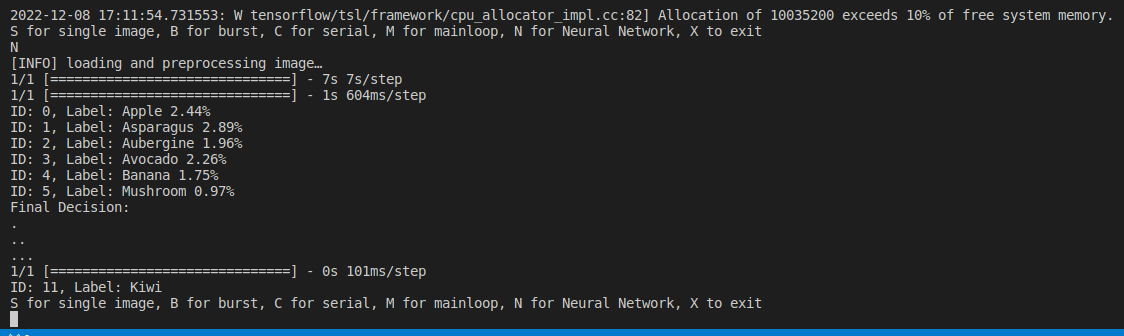
\includegraphics[width=.66\textwidth]{Ionanna.png}
    \caption{Screenshot of testing an image of label "apple"}
\end{figure} 

\subsubsection{Barcode Detection [JG]}

An important feature of the smart fridge was to identify the products placed inside it.
One of the ways in which we sought to achieve this was using a barcode detection system.
The idea for this was to find and decode barcodes found within the image received from the camera.
This would then be sent to the server to identify the product.
The code for barcode detection would be written in Python, using the OpenCV library to search the image for the barcodes, as well as any other libraries required to efficiently complete this task.
It was decided that we would use an 'off-the-shelf' algorithm as inspiration which we could later adapt to suit our needs.
Overall, three algorithms were tested in order to arrive at the best option for our product.
They were tested using three images containing barcodes.

The first image was the back of a notebook.
The idea was that this image would be the simplest as the barcode would be located on a flat, smooth surface.
A chosen algorithm would be expected to correctly detect and decode this barcode.
The second image was a barcode on a jar.
This image was intended to be more challenging as the surface of the barcode, although smooth, was no longer flat as it followed the curve of the jar.
A chosen algorithm would again be expected to detect this barcode, albeit with a lower success rate.
The third was of a barcode on a bottle.
This image was selected to be the most challenging of the three as the surface of the barcode was neither flat nor smooth.
A chosen algorithm was not required to successfully detect or decode the barcode in this image as its purpose was mainly to test the limits of each algorithm.

The first algorithm \cite{rosebrock_2021} only detected barcodes and did not decode them.
However, this was chosen as a starting point as \cite{rockikz_2020} explained the workings of the algorithm clearly and in detail.
The algorithm begins by converting the image to greyscale using the Sobel function found within the OpenCV library.
From this the x and y gradients from the Scharr operator are subtracted which gives the regions of the image which have the largest horizontal gradients and the lowest vertical gradients as these are most likely to contain barcodes within them.
The next step was to blur the image and to threshold the image, so that, pixels in which it was decided that a barcode is unlikely to be, could be set to black and pixels where a barcode was likely to be, could be set to white.
This would reduce the noise of the image in order to make the following steps easier and more effective.
The code up to this point is shown in the image below.

\begin{figure}[H]        
    \centering
    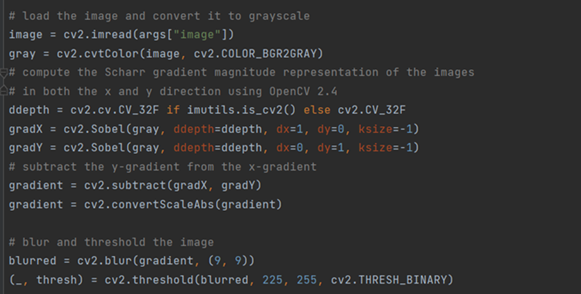
\includegraphics[width=0.5\textwidth]{Chapter 4/Barcode Detection/Figure1.png}
    \caption{Greyscaling and Blurring Code}
    \label{fig:bc1}
\end{figure} 

However, this previous step would also create gaps within the actual barcode.
Therefore, it was necessary to perform morphological operations using a rectangular kernel, once to close gaps between bars in the barcodes, and again to close any gaps within these bars.
These were then followed by four iterations of dilations which aimed to remove any remaining gaps in the barcode.
The next step was to find the largest contour in the image as this is likely the region which contains the barcode.
The code for this is shown below.

\begin{figure}[H]        
    \centering
    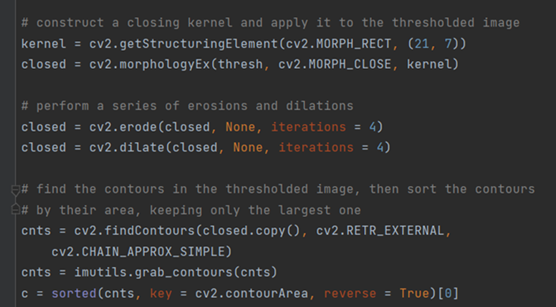
\includegraphics[width=0.5\textwidth]{Chapter 4/Barcode Detection/Figure2.png}
    \caption{Gap Closing and Contour Finding Code}
    \label{fig:bc2}
\end{figure} 

This algorithm's performance on the three test images exceeded expectations.
It was able to correctly detect the barcodes on both the notebook and the jar, however, the algorithm was also able to detect the barcode on the bottle.
Therefore, the only disadvantage of this algorithm was the missing functionality for decoding barcodes.
Due to the quality of the results, this functionality was added and tested.
Unfortunately, it was not possible for this to be implemented in a way that kept the results of the barcode detection within the time that was allocated for this algorithm.

The second algorithm \cite{ryan_zabad_vaughan_2019} added onto the first in that it included functionality for both detecting and decoding barcodes.
The sections of code dedicated to detecting the barcodes were very similar as the same method was used, with most differences being due to the use of different libraries.
However, the code for decoding the barcodes was new and therefore, the most interesting section.

As with detecting the barcode, the first step to reading the barcode was to convert the image to greyscale.
The image was then thresholded in order to identify the individual bars within the barcode.
Following this, a similar method to the previous algorithm is used to remove gaps from the barcode.
The code for this is shown below.

\begin{figure}[H]        
    \centering
    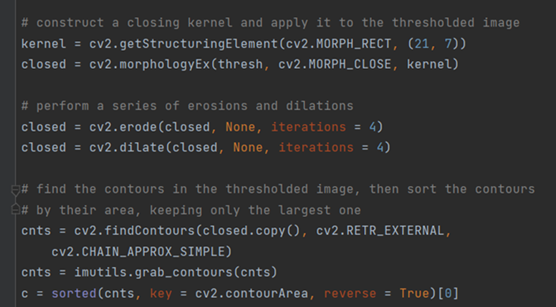
\includegraphics[width=0.5\textwidth]{Chapter 4/Barcode Detection/Figure3.png}
    \caption{Greyscaling, Thresholding and Cleaning Code}
    \label{fig:bc3}
\end{figure} 

Following this the algorithm is then able to extract the binary code from the barcode.
This is done using a separate function within the program, getBinary().
This function works by first calculating the exact boundaries of the barcode.
These are then used to iterate over the barcode as the program finds the average value of the pixels in each bar.
Then, if the average value is high, the bar is read as a '1', otherwise, the bar is read as a '0'.
In the decodeBarcode() function, the barcode is then converted from binary into the appropriate number.
The code for this is shown below.

\begin{figure}[H]        
    \centering
    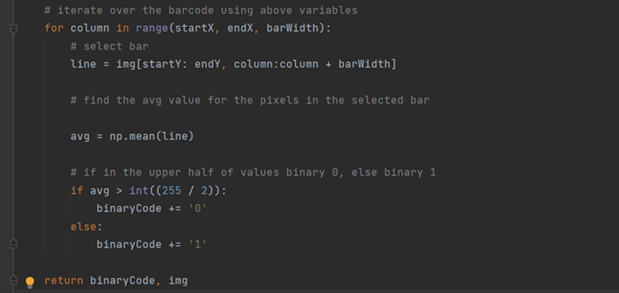
\includegraphics[width=0.5\textwidth]{Chapter 4/Barcode Detection/Figure4.png}
    \caption{Binary Extracting Code}
    \label{fig:bc4}
\end{figure} 

This algorithm's performance on the test images fell below expectations as it failed to either detect or decode the barcode in any of the three images.
It was suspected that there may have been an error in the code which caused this.
Therefore, the algorithm was tested using the test image provided by \cite{ryan_zabad_vaughan_2019}
When tested with this image the algorithm functioned properly, detecting the barcode and decoding it correctly.
In order to test whether one section of the code was working worse than the other, the barcode decoding sections of the code were implemented with the barcode detection of the previous algorithm.
However, this did not improve its performance.
Therefore, this algorithm was discarded as an option.

The third algorithm \cite{rockikz_2020} also provided functionality for both detecting and decoding barcodes.
However, this algorithm achieved this using the pyzbar library, which was designed for detecting and decoding barcodes.
As a result, the code for this third algorithm is much more condensed and easier to read.
For example, when using the pyzbar library, detecting and decoding a barcode is done with one line of code.
This is shown in the image below.

\begin{figure}[H]        
    \centering
    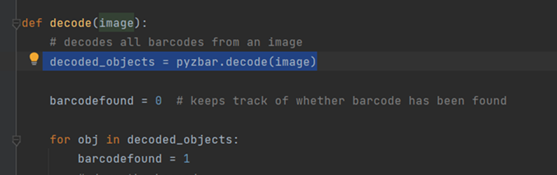
\includegraphics[width=0.5\textwidth]{Chapter 4/Barcode Detection/Figure5.png}
    \caption{Barcode Detection and Decoding Code (highlighted)}
    \label{fig:bc5} 
\end{figure} 

The program then used the glob library to iterate through files of the name “barcode*” where '*' is a number and added them to a list.
From here the program could iterate through the list, decoding the barcodes in each of these images.

This algorithm performed as expected on the tests.
It was able to both read and decode the barcode on both the notebook and the jam.
Despite this, the algorithm was unable to either detect or decode the barcode on the bottle, however, given the challenging condition of that barcode, this was not a requirement for an algorithm to be chosen.
The results for each test are shown below.

\begin{figure}[H]        
    \centering
    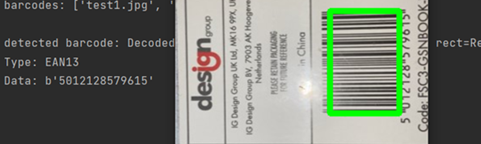
\includegraphics[width=.66\textwidth]{Chapter 4/Barcode Detection/Figure6.png}
    \caption{First Result}
    \label{fig:bc6} 
\end{figure} 

\begin{figure}[H]        
    \centering
    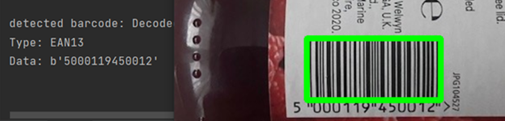
\includegraphics[width=.66\textwidth]{Chapter 4/Barcode Detection/Figure7.png}
    \caption{Second Result}
    \label{fig:bc7} 
\end{figure} 

\begin{figure}[H]        
    \centering
    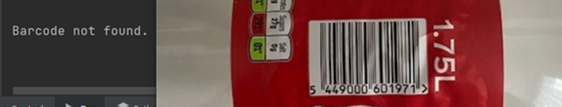
\includegraphics[width=.66\textwidth]{Chapter 4/Barcode Detection/Figure8.png}
    \caption{Third Result}
    \label{fig:bc8} 
\end{figure} 


Given the results shown in figures 6-8, this algorithm was chosen for use in our product.
In its original state, the algorithm already satisfied most of the product's needs as it could decode barcodes from an image.
However, it was necessary to add an error message for cases where the barcode could not be decoded.
The first step was to declare a variable, 'barcodefound', at the start of the decode() function and set it equal to 0.
This variable would later tell us whether a barcode had been decoded.
Then, in the for loop within the same function, this variable would be changed to 1.
This worked because the program would only enter the loop if there were items in the decoded\_objects list.
As each item in this list was a barcode, if this list was empty, a barcode was not found within the image and, therefore, the 'barcodefound' variable would remain unchanged.
However, if there was at least one item in the list, 'barcodefound' was changed to 1.
This was then followed by an if statement to check the value of 'barcodefound'.
If this was still equal to 0, a message was printed to the terminal.
This can be seen in figure 8, with the code shown below.

\begin{figure}[H]        
    \centering
    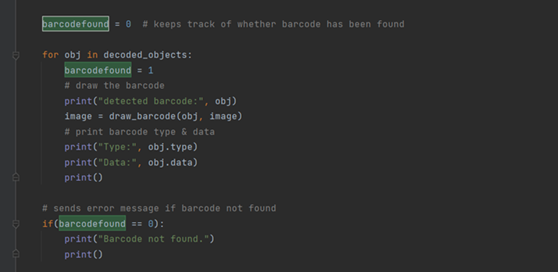
\includegraphics[width=.66\textwidth]{Chapter 4/Barcode Detection/Figure9.png}
    \caption{Error Checking Code}
    \label{fig:bc9} 
\end{figure} 

\subsubsection{Pi Camera [AW]}

A USB camera is plugged into the Raspberry Pi.
Using the OpenCV library to access the camera, pictures can be taken and then analyzed by the previously discussed computer vision methods.
The webcam being used is not perfect but is suitable for a first prototype.
It is unable to have its focus adjusted programmatically so the camera will have to be focused manually when being fitted into the enclosure.

This is fine for now but in the future, it would be appropriate to replace the webcam with a different camera that allows for focus to be adjusted automatically and is more suited to fitting within the housing of a fridge.
By doing this, the reliability of extracting barcodes and expiration dates would increase due to having higher clarity images.

\begin{figure}[H]        
    \centering
    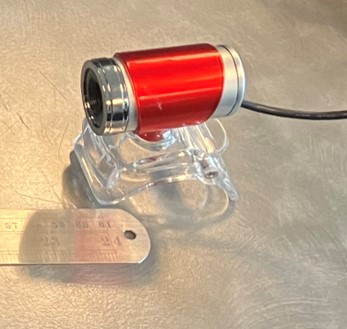
\includegraphics[width=0.5\textwidth]{Chapter 4/Pi Camera/ImageOfWebcam.jpg}
    \caption{Webcam}
    \label{fig:webcam} 
\end{figure} 

The images are stored in a bitmap image file, known as BMP for short.
This is done to maintain a high-resolution image as opposed to the JPEG file format.
Figure \ref{fig:webcampic} shows an image from the camera on the raspberry pi.

Since the original design intended for an ESP32 camera to be used, the webcam was a backup idea that had to be utilized with the time left.
Fortunately, the Pi is perfectly suited to handling the camera since the open cv library is already a requirement and the goal was to transfer the image from the ESP-32 to the Pi regardless.
Ultimately, it has increased the complexity of the wiring while decreasing the complexity of the ESP-32 and Raspberry Pi code.

\begin{figure}[H]        
    \centering
    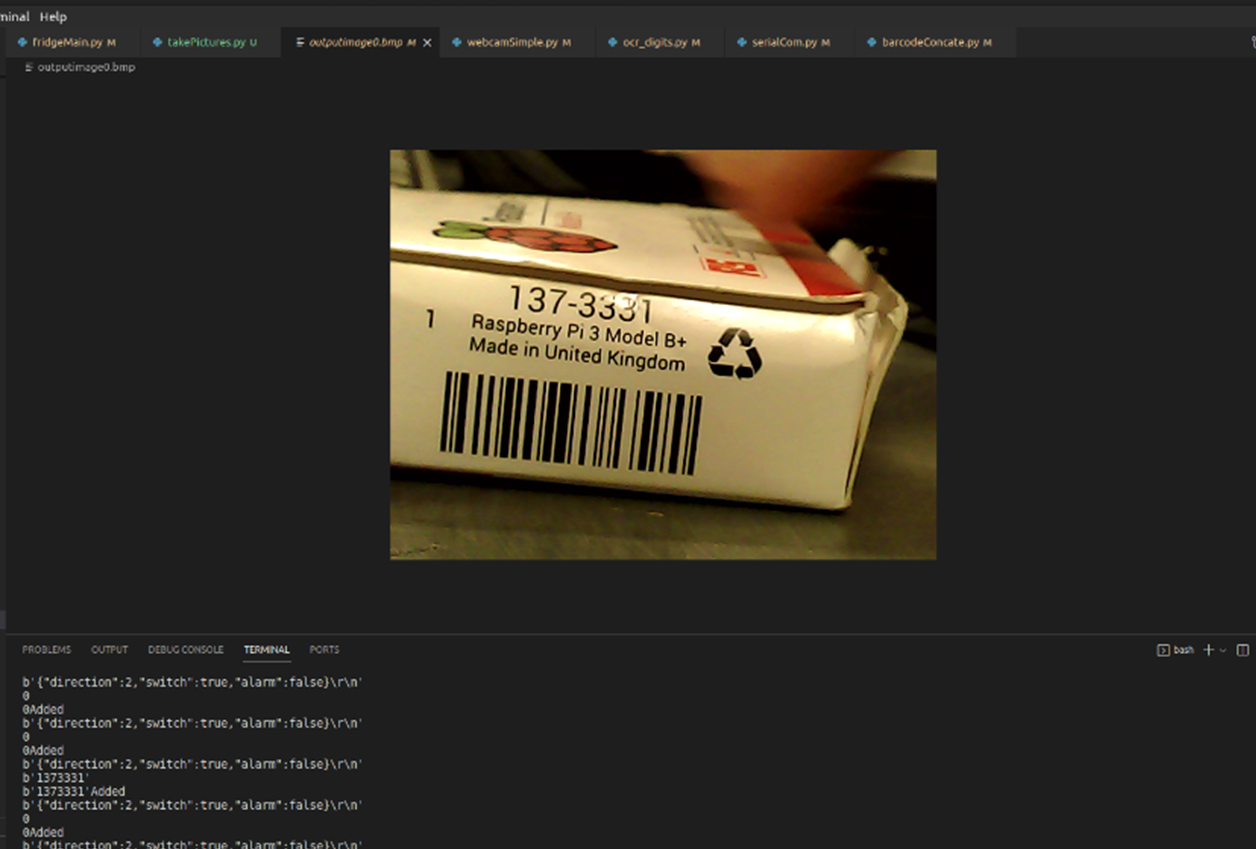
\includegraphics[width=.66\textwidth]{Chapter 4/Pi Camera/PiBoxTakenByCamera.png}
    \caption{Picture from Webcam}
    \label{fig:webcampic} 
\end{figure} 

In figure \ref{fig:webcampic} a picture taken by the webcam of the Raspberry Pi box barcode can be seen.
In the terminal the byte value of b'1373331' is detected which matches the number written on the box.

\subsubsection{Pi Serial Input [AW]}

To communicate between the ESP-32 and Raspberry Pi, the serial RX and TX pins are connected.
As seen on the pinout \ref{fig:rpigpio}, the GPIO 14 (TXD) pin is used to transmit data and the GPIO 15 (RXD) pin is used to receive data.

\begin{figure}[H]        
    \centering
    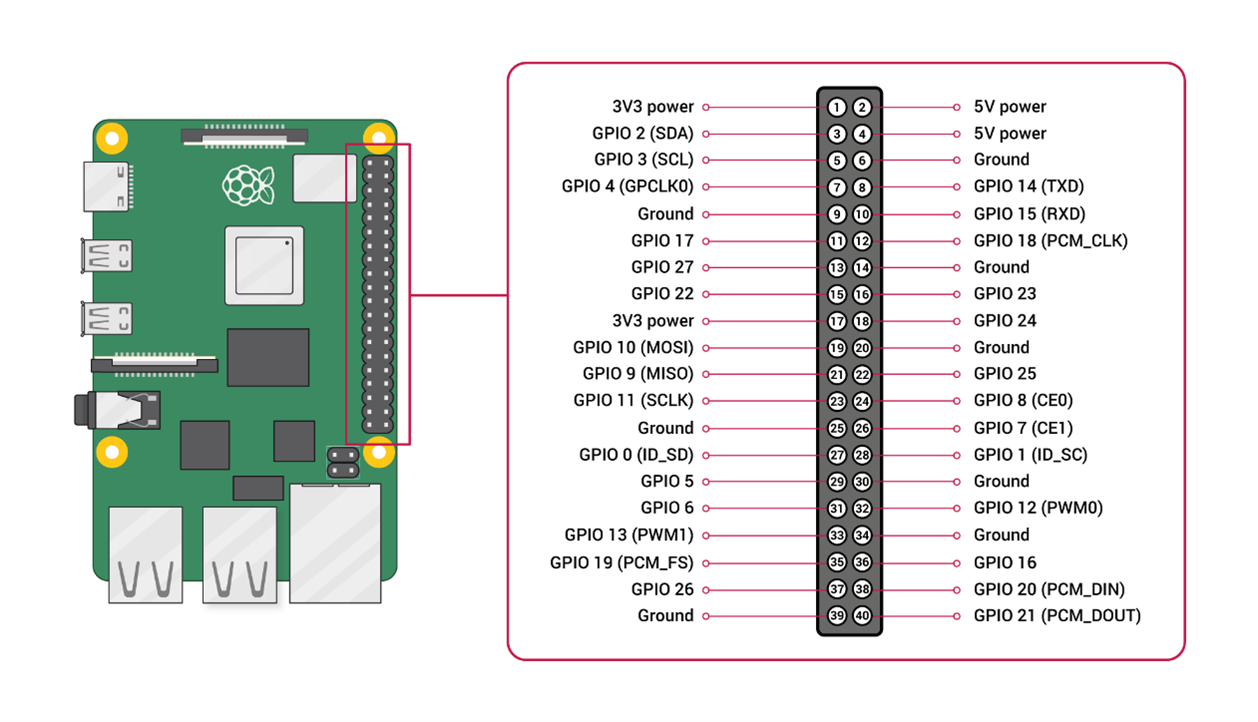
\includegraphics[width=.66\textwidth]{Chapter 4/Serial Input/PiPinout.png}
    \caption{GPIO of the RPI}
    \label{fig:rpigpio} 
\end{figure} 

The information received will be a JSON file containing the status of the door, the direction of movement and if the alarm is sounding.
The JSON format table can be seen in table \ref{tab:yohan}

The ESP-32 was connected to the Raspberry Pi by using two jumper wires to test if the serial input was functional and as seen in \ref{fig:rpiserial}

\begin{figure}[H]        
    \centering
    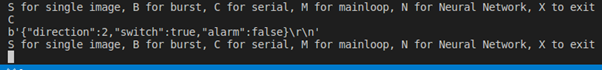
\includegraphics[width=1\textwidth]{Chapter 4/Serial Input/SerialRead.png}
    \caption{Serial Data from ESP}
    \label{fig:rpiserial} 
\end{figure} 

The message received was: “b'{“direction”:2,”switch”:true,”alarm”:false} r n”

Which means that an item is entering the fridge, while the door is open and the alarm is not sounding.

\subsubsection{Pi Communications [ASH]}

For the PI to function it needs to read known items from the database as well as add and remove instances of the items from people's inventory.
Supabase, our back-end, provides a python API to interact with the tables as well as to handle user authentication.
However for ease of use for the Pi Software team multiple functions were designed to simplify and abstract the database commands and manage the database connection in the background.
These key functions allow the PI to: retrieve items, add items to the inventory, remove items from the inventory and log the user in.

This was done by creating a class that expands on the provided “Client” class from the Supabase python API.
The Client class exposes the same commands as the JS commands and allows the user to perform various actions, however for the RPI side of the communication we are only concerned with interacting with the database.
The commands exposed by Supabase require syntax similar to the SQL command used to drive the database directly, however as mentioned we wanted to abstract these so the SQL commands and code required to package items as JSON have been wrapped into simple commands to getItemID, addItem, and removeItem.
The class also deals with logging the user in, ensuring we can access the user's data, and subsequently logging out when appropriate.
All these functions were tested with a simple unit test that would log in, check items, add items, remove items, get a barcode, and log out.

As with the rest of the code base, the communication section was created entirely separately from the main code base meaning that the initial structure was rather different and integration was required.
These changes were later unified in the code refactor.
After this refactor the database code worked well with the rest of the code base, and, as the API is similar in python and JavaScript, the experience of writing this code was easily transferred to creating the App.

\subsubsection {Pi Integration [AW]}

The main bulk of integration is sitting down with the team members who worked on their individual sections while moving the python code to the Raspberry Pi environment.
This ensures that the transition is smooth and that issues are solved as quickly as possible.

% Please add the following required packages to your document preamble:
% \usepackage{longtable}
% Note: It may be necessary to compile the document several times to get a multi-page table to line up properly
\small
% Please add the following required packages to your document preamble:
% \usepackage{longtable}
% Note: It may be necessary to compile the document several times to get a multi-page table to line up properly
\begin{longtable}[c]{|l|l|l|}
\caption{Overview of Python Libraries}
\label{tab:libraries}\\
\hline
Module/Library &
  Section &
  Function \\ \hline
\endfirsthead
%
\endhead
%
serial &
  Serial Communication &
  \begin{tabular}[c]{@{}l@{}}Enables Serial communication on\\ the GPIO 14 pin for transmitting\\ and GPIO 15 pin for receiving.\end{tabular} \\ \hline
cv2 &
  \begin{tabular}[c]{@{}l@{}}Barcode, Optical character\\ recognition\end{tabular} &
  \begin{tabular}[c]{@{}l@{}}Cv2 is the Open CV library for python.\\ It lays the foundation for computer\\ vision code in the project as well as\\ the image handling.\end{tabular} \\ \hline
io &
  \begin{tabular}[c]{@{}l@{}}Barcode, Serial Communication, \\ Optical character recognition\end{tabular} &
  \begin{tabular}[c]{@{}l@{}}The io module provides pythons\\ main methods for dealing with inputs\\ and outputs.\end{tabular} \\ \hline
time &
  CNN, Barcode &
  \begin{tabular}[c]{@{}l@{}}The time library is used to add delay\\ during the image processing.\end{tabular} \\ \hline
json &
  Serial Communication &
  \begin{tabular}[c]{@{}l@{}}The JSON library is used to convert\\ the JSON received from the ESP\\  into readable values.\end{tabular} \\ \hline
pyzbar &
  Barcode &
  \begin{tabular}[c]{@{}l@{}}Pyzbar is the library that handles\\ decoding and detecting barcodes in \\ images.\end{tabular} \\ \hline
pytesseract &
  Optical character recognition &
  \begin{tabular}[c]{@{}l@{}}Pytesseract is the library that handles\\ decoding and detecting characters in \\ images.\end{tabular} \\ \hline
pandas &
  CNN product recognition &
  \begin{tabular}[c]{@{}l@{}}The pandas library is used for data\\ analysis.\end{tabular} \\ \hline
numpy &
  CNN product recognition &
  \begin{tabular}[c]{@{}l@{}}The NumPy module allows python\\ to use high level mathematical functions \\ and operate with large multi-dimensional\\ arrays and matrices.\end{tabular} \\ \hline
shutil &
  CNN product recognition &
  \begin{tabular}[c]{@{}l@{}}Shutil allows the python program to \\ do high level operations on files.\end{tabular} \\ \hline
itertools &
  CNN product recognition &
  \begin{tabular}[c]{@{}l@{}}The Itertools module implements \\ functions to increase the efficiency \\ of loops in the code.\end{tabular} \\ \hline
tensorflow &
  CNN product recognition &
  \begin{tabular}[c]{@{}l@{}}The TensorFlow module used to prepare\\ and load data for machine learning.\end{tabular} \\ \hline
keras &
  CNN product recognition &
  \begin{tabular}[c]{@{}l@{}}Keras provides an open-source software\\ library that acts as an interface for \\ TensorFlow.\end{tabular} \\ \hline
sklearn &
  CNN product recognition &
  \begin{tabular}[c]{@{}l@{}}Sklearn (or scikit-learn) features\\ classification, regression, and clustering\\ algorithms to be used with machine learning.\end{tabular} \\ \hline
\end{longtable}

These modules were installed using “pip install” on the Linux environment on the Pi.

Once all the required modules were installed, the code from other group members must be compiled into a main loop to run on the Pi.
On the other hand, each part must be tested individually first.
This was done by creating a simple loop that asks the user which section they want to run.

\begin{figure}[H]        
    \centering
    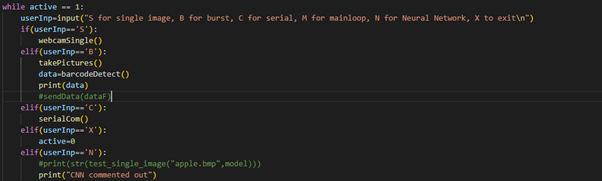
\includegraphics[width=1\textwidth]{Chapter 4/Pi Integration/PiTestLoop.png}
    \caption{Test Loop Code}
    \label{fig:tlcode}
\end{figure} 

As seen in figure \ref{fig:tlcode} the letter S can be input to take a single image and check for barcodes, the letter B to check a burst of images for barcodes, the letter C to test the serial input from the ESP-32, N to test the neural network on an image and X to cancel the program and exit.
This allows the core base functionality to be tested individually before the final implementation.

\subsubsection {Code Refactor [ASH, AW]}

As is inevitable when code is written by many different people, in particular when the overall design is not determined before coding begins, our code base was somewhat inconsistent, poorly formatted, and used different conventions.
To allow us to iterate and improve the code faster once the different sections, such as the barcode recognition, produce detection, and database iterations were combined, we took the time to refactor the code into something of a more unified and thought-out design.

The first step in the refactor was simply to remove all the unused code (including imports), debug images, and other files left behind from testing.
This alone already made large improvements to the readability of the code and allowed us to start making decisions such as what format to use and how to restructure the code.
Other, more superficial changes,  were also made.
These changes included setting up a “.gitignore” file to clean up the repository and a requirements file to help set up the requirements on new machines

After this initial clean-up, we decided to rework the code in a more object-oriented style, similar to how the Supabase communication section was initially written.
While doing this we also tried to adopt a more consistent naming scheme for both function and member variables.
This was done to unify the style of each section, making the code much easier to understand and edit.
We settled for the design seen below in figure \ref{fig:oocd}, table \ref{tab:piview} provides more detail on these member functions and variables.

\begin{figure}[H]        
    \centering
    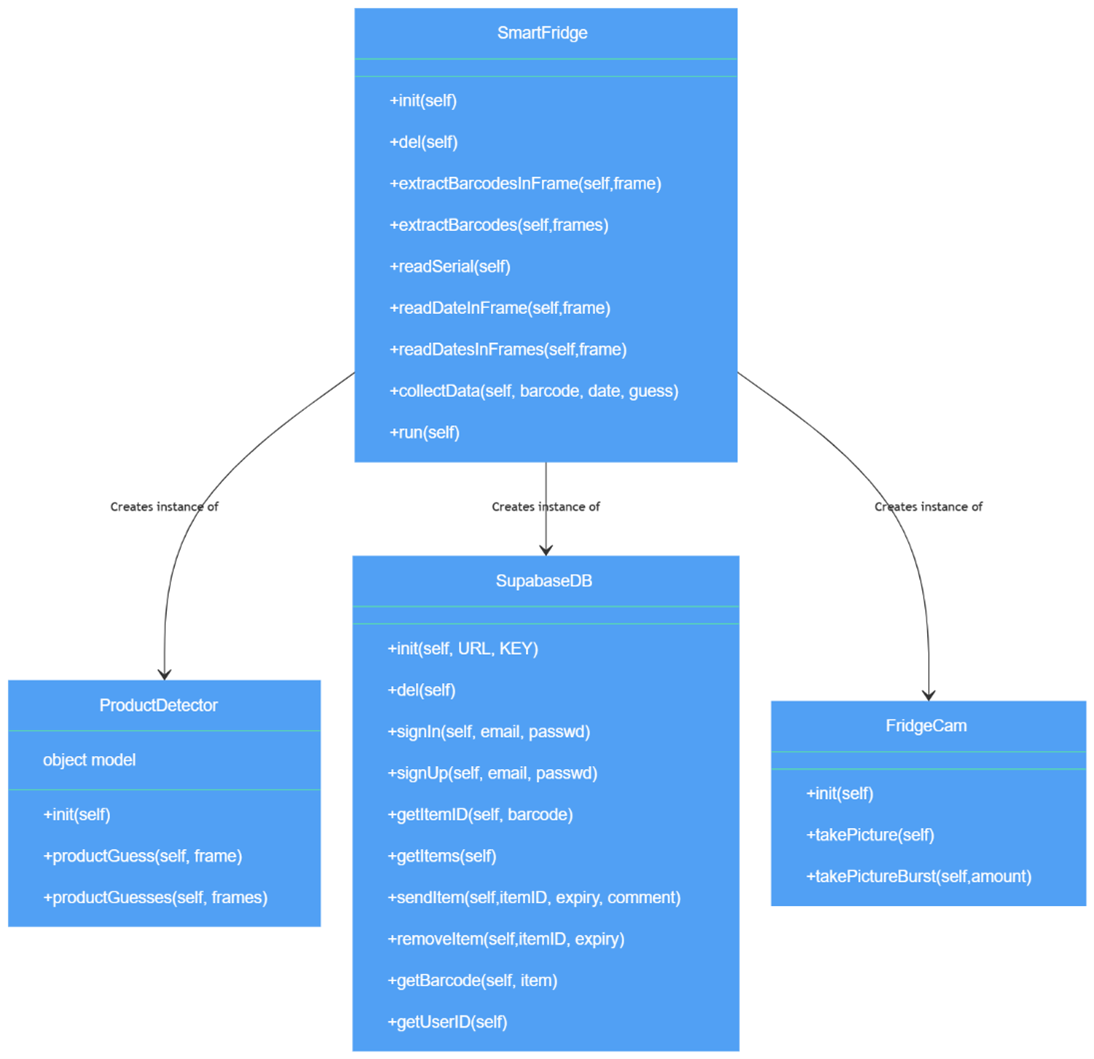
\includegraphics[width=.66\textwidth]{Chapter 4/Code Refactor/Class Diagram.png}
    \caption{Object Oriented Class Diagram}
    \label{fig:oocd}
\end{figure} 

Now the fridge's core operations were encompassed in a single object, which itself contains instances of the objects that simplify and abstract the usage of the CNN product detector, Supabase database connection, and camera.
After this major refactor, we also changed the layout of the python files themselves, placing them in a Smart Fridge directory with an “\_\_init\_\_.py” file which is required for the code to show up as a module.
This allows us to cleanly import all our code into a short-run file which will start everything we need for the Smart Fridge's local operation.

While it would have been preferable to have never needed to refactor, this would have slowed initial programming down and would have required many assumptions about what choices would be made by other people on the team.
As effort would have been required to integrate the code regardless, doing this refactor allowed us to examine our code as well as improve it as we went along.
Testing for this was rather simple, as the end goal was essentially to maintain the same functionality as before, meaning the same test could be run.
This refactor was a success as we managed to improve the code slightly with some optimizations all the while making it much more readable and easier to set up on another device.

% Please add the following required packages to your document preamble:
% \usepackage{longtable}
% Note: It may be necessary to compile the document several times to get a multi-page table to line up properly
\begin{longtable}[c]{|l|l|}
    \caption{Python Class and Method Overview}
    \label{tab:piview}\\
    \hline
    \textbf{Method/Class} &
      \textbf{Explanation} \\ \hline
    \endfirsthead
    %
    \endhead
    %
    \textbf{ProductDetector Class} &
      \textbf{\begin{tabular}[c]{@{}l@{}}Class that handles the neural network \\ algorithm.\end{tabular}} \\ \hline
    init(self) &
      \begin{tabular}[c]{@{}l@{}}Initializes the neural network by loading\\  in the weights, and  layers of the model.\end{tabular} \\ \hline
    productGuess(self,frame) &
      \begin{tabular}[c]{@{}l@{}}Runs the neural network on the image (frame) \\ passed into the method and returns the name \\ of the product guessed.\end{tabular} \\ \hline
    productGuesses(self, frames) &
      \begin{tabular}[c]{@{}l@{}}Runs productGuess on all the images (frames) \\ passed into the  method.\end{tabular} \\ \hline
    FridgeCam Class &
      Class that handles taking pictures on the webcam. \\ \hline
    init(self) &
      \begin{tabular}[c]{@{}l@{}}Initializes the camera so it can be accessed by\\ open cv.\end{tabular} \\ \hline
    takePicture(self) &
      Takes a picture and returns it. \\ \hline
    takePictureBurst(self, amount : int) &
      \begin{tabular}[c]{@{}l@{}}Takes several pictures equal to the value of\\ amount.\end{tabular} \\ \hline
    \textbf{SupabaseDB Class} &
      \textbf{\begin{tabular}[c]{@{}l@{}}Connects to the supabase database and sends\\ data to it.\end{tabular}} \\ \hline
    init(self, URL, KEY) &
      Initializes the user key and user ID. \\ \hline
    del(self) &
      Signs out the user. \\ \hline
    signIn(self, email, passwd) &
      Log into existing user. \\ \hline
    signUp(self, email, passwd) &
      Create a new user. \\ \hline
    getItemID(self, barcode) &
      \begin{tabular}[c]{@{}l@{}}Takes in a barcode as an argument and\\ returns the item ID that  represents that item.\end{tabular} \\ \hline
    getItems(self) &
      Gets all the user’s items in the fridge. \\ \hline
    sendItem(self, itemID, expiry, comment) &
      \begin{tabular}[c]{@{}l@{}}Sends an item to be stored in the database\\ by using the item ID,   the expiry date, and an\\ additional comment.\end{tabular} \\ \hline
    removeItem(self, itemID, expiry) &
      \begin{tabular}[c]{@{}l@{}}Removes an item from the database, taking\\ itemID and expiry data  as parameters.\end{tabular} \\ \hline
    getBarcode(self,item) &
      \begin{tabular}[c]{@{}l@{}}Returns the barcode value based on the item\\ parameter (itemID).\end{tabular} \\ \hline
    getUserID(self) &
      Returns UserID of the current fridge user \\ \hline
    \textbf{SmartFridge Class} &
      \textbf{\begin{tabular}[c]{@{}l@{}}Contains the main loop for the fridge and\\ connects all the other  sections/modules.\end{tabular}} \\ \hline
    init(self) &
      \begin{tabular}[c]{@{}l@{}}Initialize instance of ProductDetector,\\ FridgeCam and SupabaseDB, declare the\\ baud rate to match the ESP32 and set the\\ options for the optical character recognition.\end{tabular} \\ \hline
    del(self) &
      Closes the serial port. \\ \hline
    extractBarcodesInFrame(self, frame) &
      \begin{tabular}[c]{@{}l@{}}Takes in a frame (image) as a parameter\\ and identifies and reads  any barcodes in\\ the image. Returns the barcodes at the\\ end of the method.\end{tabular} \\ \hline
    extractBarcodes(self,frames) &
      \begin{tabular}[c]{@{}l@{}}Takes in frames (multiple images) as a\\ parameter and calls extractBarcodesInFrame\\  on each of them. It then returns a list of\\ found barcodes.\end{tabular} \\ \hline
    readSerial(self) &
      \begin{tabular}[c]{@{}l@{}}Reads data sent from the ESP-32 on the\\ serial pins and converts it from JSON into\\ an object with several string attributes.\end{tabular} \\ \hline
    readDateInFrame(self,frame) &
      \begin{tabular}[c]{@{}l@{}}Searches the passed in frame(image) for\\ readable text (optical character recognition)\\ and then returns a list of found strings.\end{tabular} \\ \hline
    readDatesInFrame(self,frames) &
      \begin{tabular}[c]{@{}l@{}}Runs readDateInFrame on each individual\\ frame (image) passed into  the method. \\ Returns a list of strings.\end{tabular} \\ \hline
    collectData(self,barcode,data,guess) &
      \begin{tabular}[c]{@{}l@{}}Constructs a list made up of the passed \\ in barcode value, date,  and guess. \\ Returns the new list.\end{tabular} \\ \hline
    run(self) &
      Contains the main loop of the SmartFridge \\ \hline
    \end{longtable}


\subsection{Back-End [ASH]}

To present the user with the content of their Smart Fridge in an app and/or website the relevant data needs to be stored somewhere that is always accessible.
While this data could be stored and transmitted locally from the Smart Fridge, this would either require that the user to be on their local area network to access the data, which is restrictive, or for that the Smart Fridge to be accessible beyond the local area network, which requires more complicated networking and could cause network security risks.
Furthermore, the client brief requires data transmission to “a known free secure location” leading us to use a cloud solution.

We chose to use Supabase, a platform utilizing open-source technologies for creating mobile and web applications, which integrates a cloud database, user authentication, easy APIs, and more.
Supabase's database is a relational database, which consists of various tables where every entry has a unique ID.
Supabase was chosen as it offers easier migrations, as well as the option of self-hosting when compared to competitors, such as AWS Amplify and Firebase, as the underlying software is open source.
Furthermore the a relation database was preferred to the No-SQL approach taken by Firebase.

For the Smart Fridge, we made use of three tables; the first table contains a list of possible items, each of them with a unique ID, the barcode value, item name, comment, and an image.
This table is used by the Raspberry Pi in the Smart Fridge to look up what items it has scanned.
Every user has read access to these values and for this prototype, the table will be populated by us with common items.
The second table contains the details of each user (we have one user per fridge), which consists primarily of their email and user ID.
Some additional data such as the last login time and date is also stored.
As well as a password hash used for login.
Besides login, users can not access this data and for this prototype, only “dummy” users with fictional emails are used.
This table is also part of Supabase's built-in “auth” scheme.
Our third, and primary, the table is where we store the actual inventory of the users.
The table contains instances of the items, where each row has the item's id from the previous table, the associated user ID, expiry date, and possible comments.
We have set up Supabase database rules, using Row Level Security, to ensure users can only request rows (which represent the individual items) from this table when the user ID column matches their user's ID, ensuring that people cannot access other people's data.
Tables one and three create our public scheme and can be seen below in Figure \ref{fig:DB_Diagram}.

\begin{figure}[H]        
    \centering
    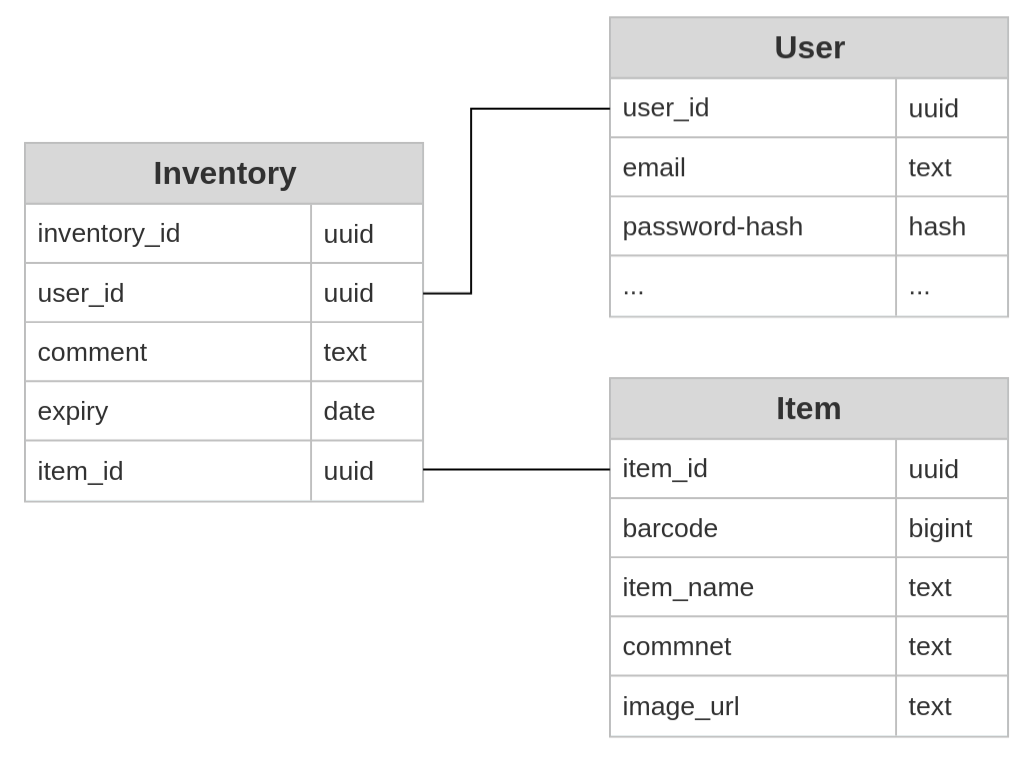
\includegraphics[width=1\textwidth]{Chapter 3/alexandre/db.png}
    \caption{DB Diagram}
    \label{fig:DB_Diagram}
\end{figure} 

Using Supabase made our database easy to set up and use, and the API provided both in JavaScript and python made interaction simple for both the Smart Fridge itself as well as the website and app.
However, one disadvantage of Supabase is the lack of hosting for our Front Ends, meaning that we need to host them separately.
This aside, the back end worked exactly as intended and provided a secure location to transmit data to.

\subsection{App [ASH]}

Smartphones are owned by over 80\% \cite{stat} of all UK adults and with that apps have become the way people interact with many facets of modern life.
This why we decided to also allow the user to access the Smart Fridge via an app, alongside the website, both of these services provide the user with the inventory of their Fridge and feed into APIs to provide insights.
While much of the core functionality overlaps with a website, the app needs to be designed very differently to work on a smartphone however the medium also provides opportunities such as sending notifications to the user as well as having a camera connected directly to the device.
With this in mind, we planned to create an app that had all the core functionality of the website: viewing the inventory, making updates to the inventory, seeing insights about the inventory such as recipe recommendations and nutritional data, and dealing with user authentication.
The app will also expand on this by providing notifications based on expiration, informing the user when the fridge is left open.

React Native, Meta's mobile app development platform using the extremely popular React JavaScript user interface framework, was our natural choice for an app.
This is because React Native is used to creating mobile apps for countless companies, ranging from Fortune 500s and start-ups \cite{react}, meaning it is powerful and versatile enough to create anything we require.
Having prior experience in React also reduced the learning curve required to make this app.
Furthermore, as React Native is based on React, often used to create websites, code between the app and website could have been shared.
Eventually, however, the decision was made to have the website written in python, regardless React Native can still render as a website meaning we also have an alternative website that works well on desktop and mobile.

The core functionality of the app is mostly supported by two external systems: the Supabase library, which allows for quick and easy connection to our back end, and the Edamam API.
The Supabase library allows us easily create a connection to the database, allowing us to handle user logins and database look-ups and updates.
There is also functionality to subscribe to events on the database, meaning the app will update without needing a manual refresh when an item is added to the Fridge.
Login also supports the “OAuth” standard, allowing users to connect using a long list of accounts such as their Google or Facebook login, however, this was disabled for the prototype as we only used dummy accounts with passwords.
The Edamam API provides the nutritional analysis and recipe search functionality of the app.
The API is very powerful and claims to contain the nutritional data of close to 900,000 foods and to have over 2.3 million recipes \cite{edman}.
More information about the API is in the section covering the website.
This alongside the natural language processing on their end allows us to send over a list of the user items, as well as attached comments containing further information about the item such as brand or unit, and receive high-quality data as a response.
These responses can then be displayed to the user.

The Smart Fridge app consists of three primary screens, pictured below in figure \ref{fig:app}.

\begin{figure}[H]
    \begin{subfigure}{.33\textwidth}
      \centering
      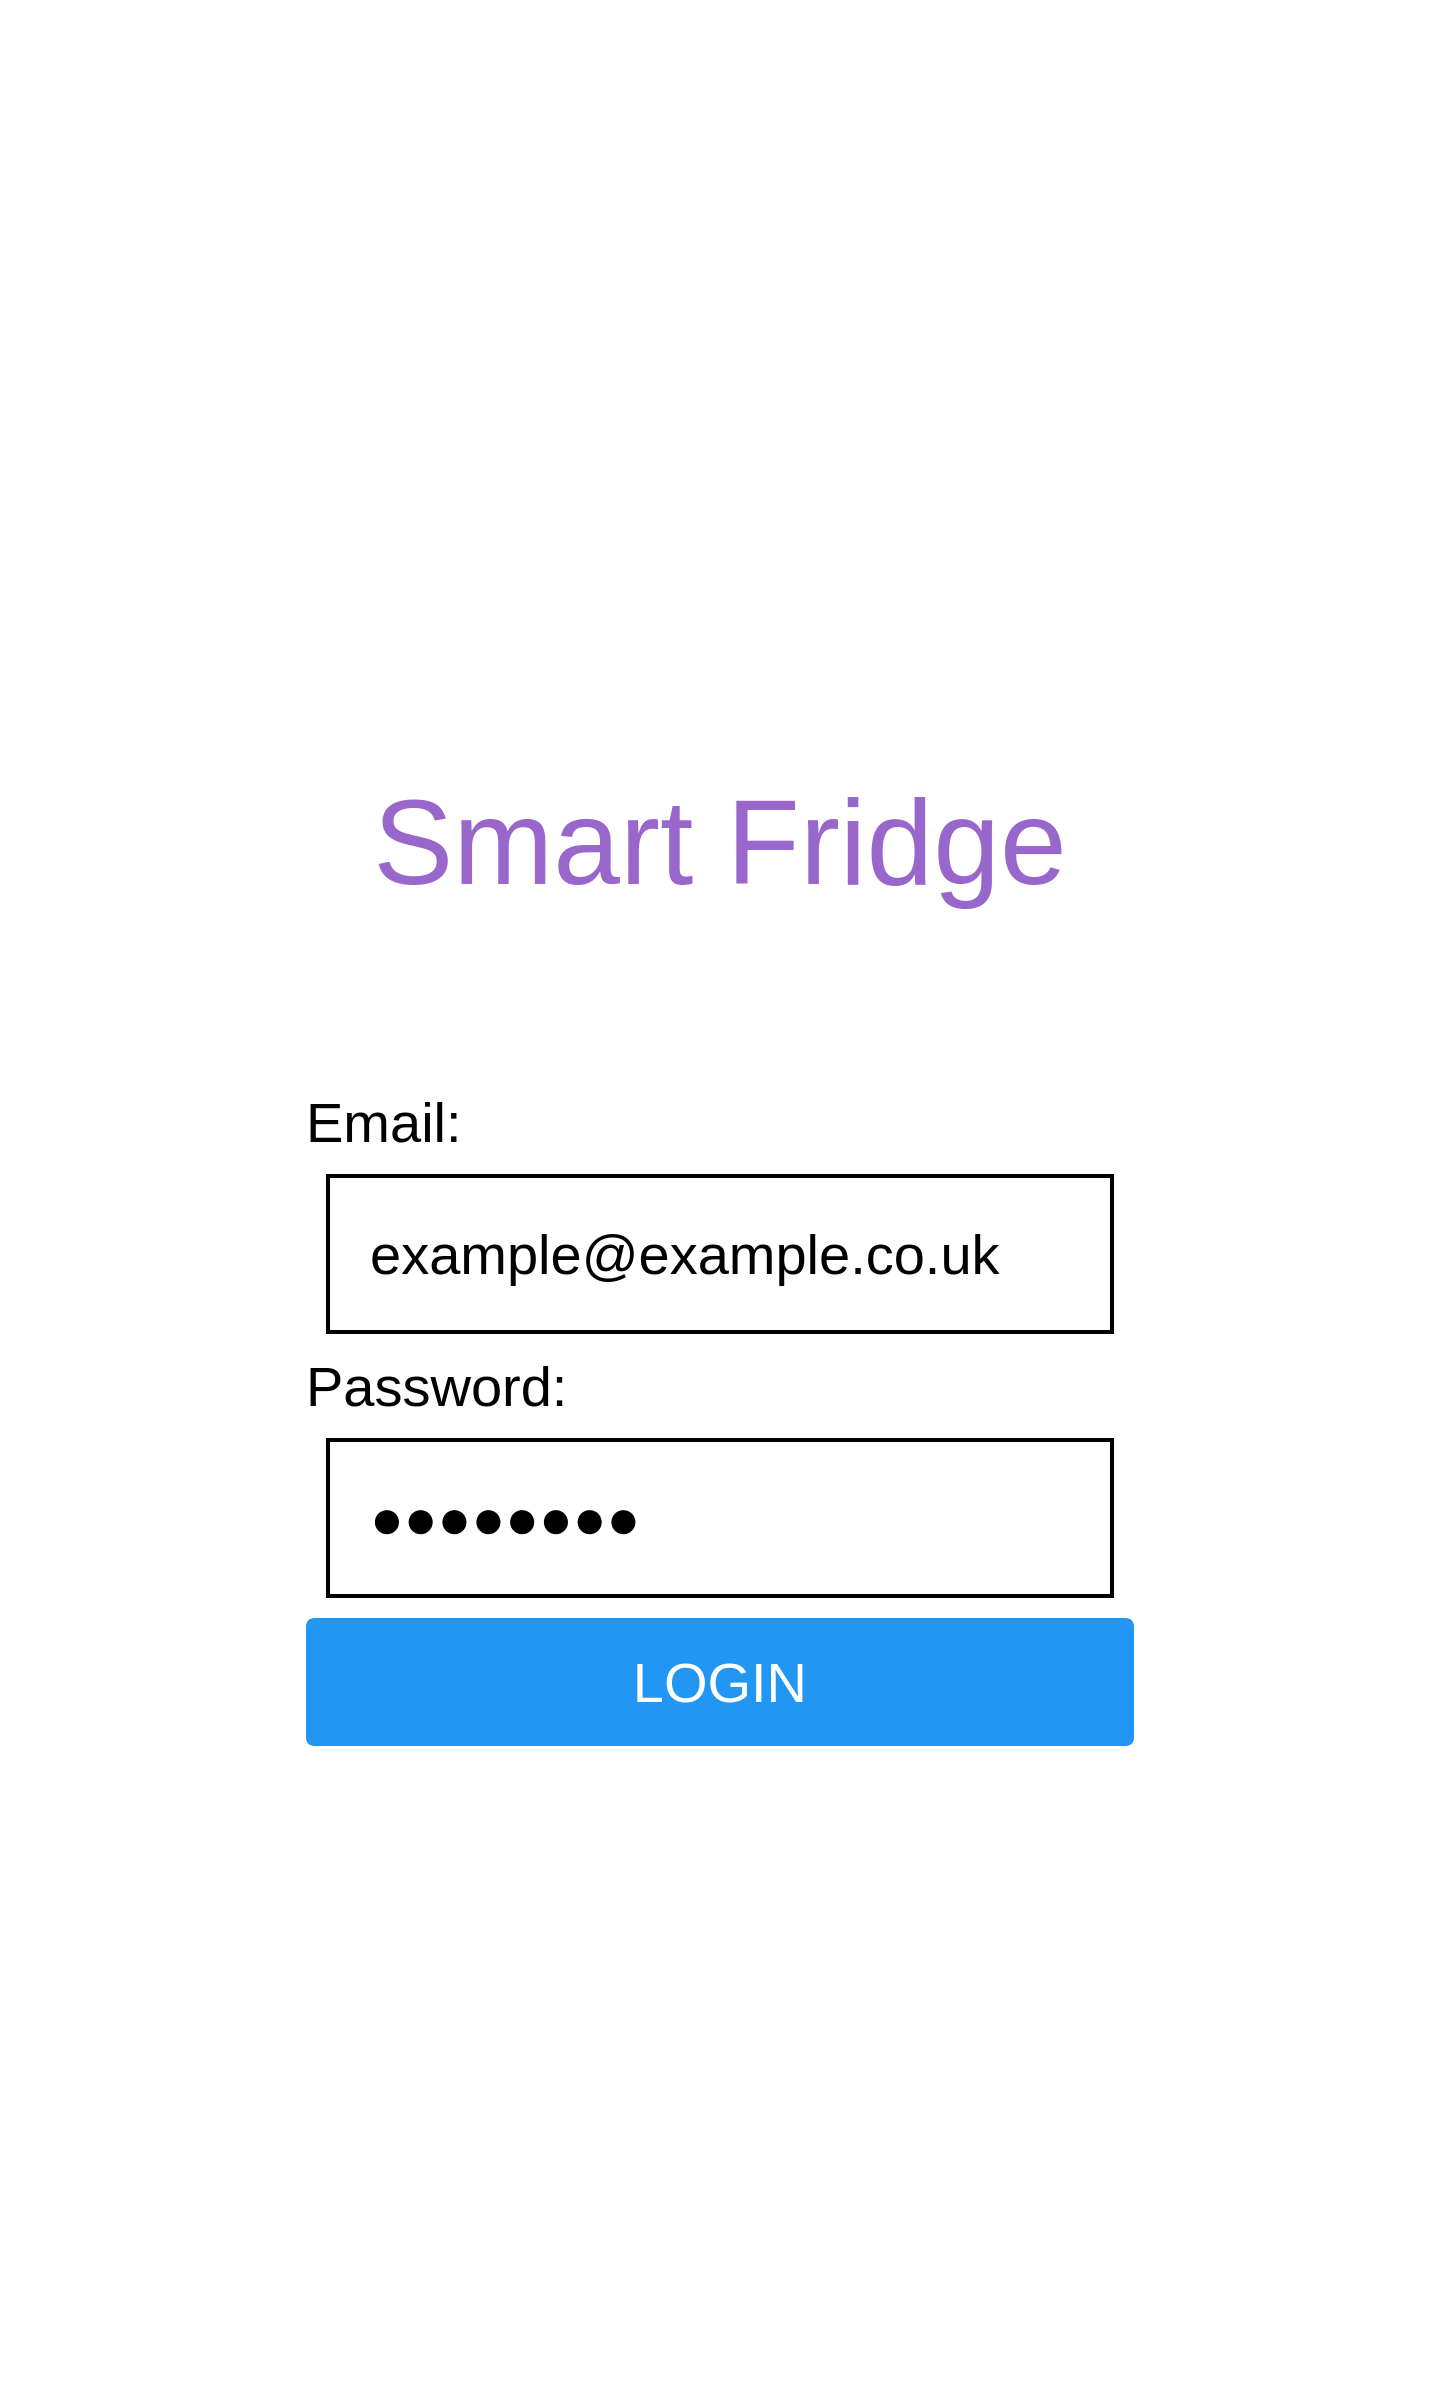
\includegraphics[width=.8\linewidth]{Chapter 4/app_pic/Login.png}
    \end{subfigure}%
    \begin{subfigure}{.33\textwidth}
      \centering
      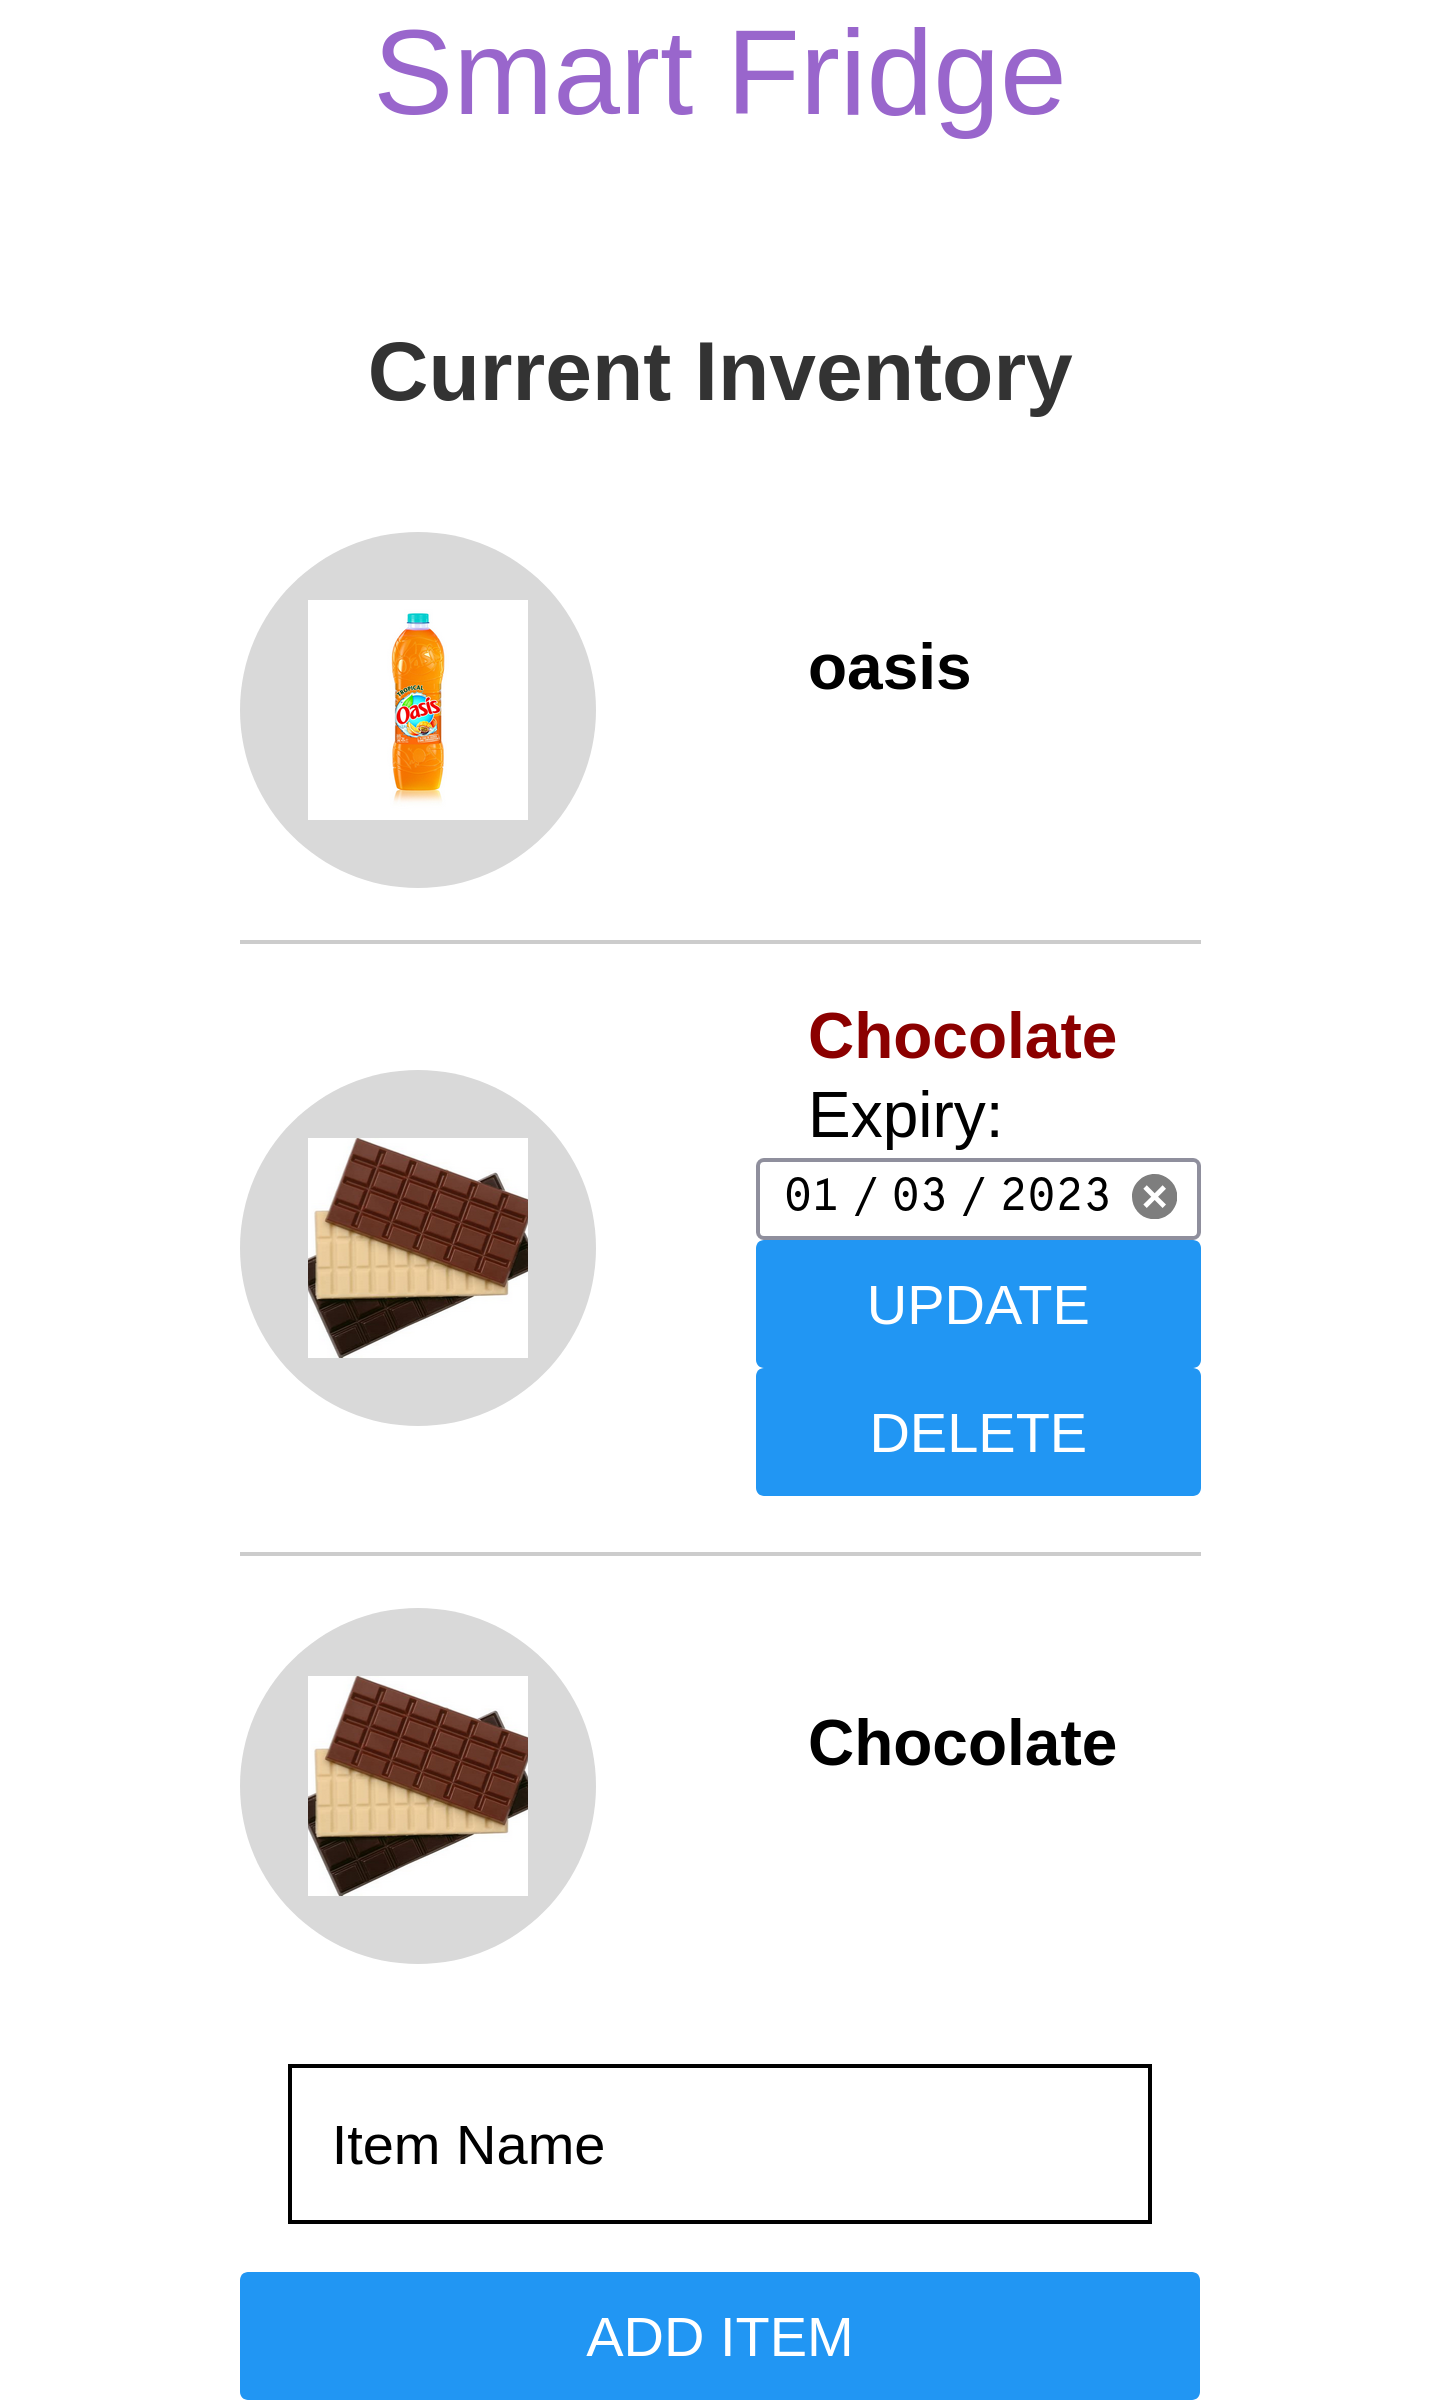
\includegraphics[width=.8\linewidth]{Chapter 4/app_pic/Inv.png}
    \end{subfigure}
    \begin{subfigure}{.33\textwidth}
        \centering
        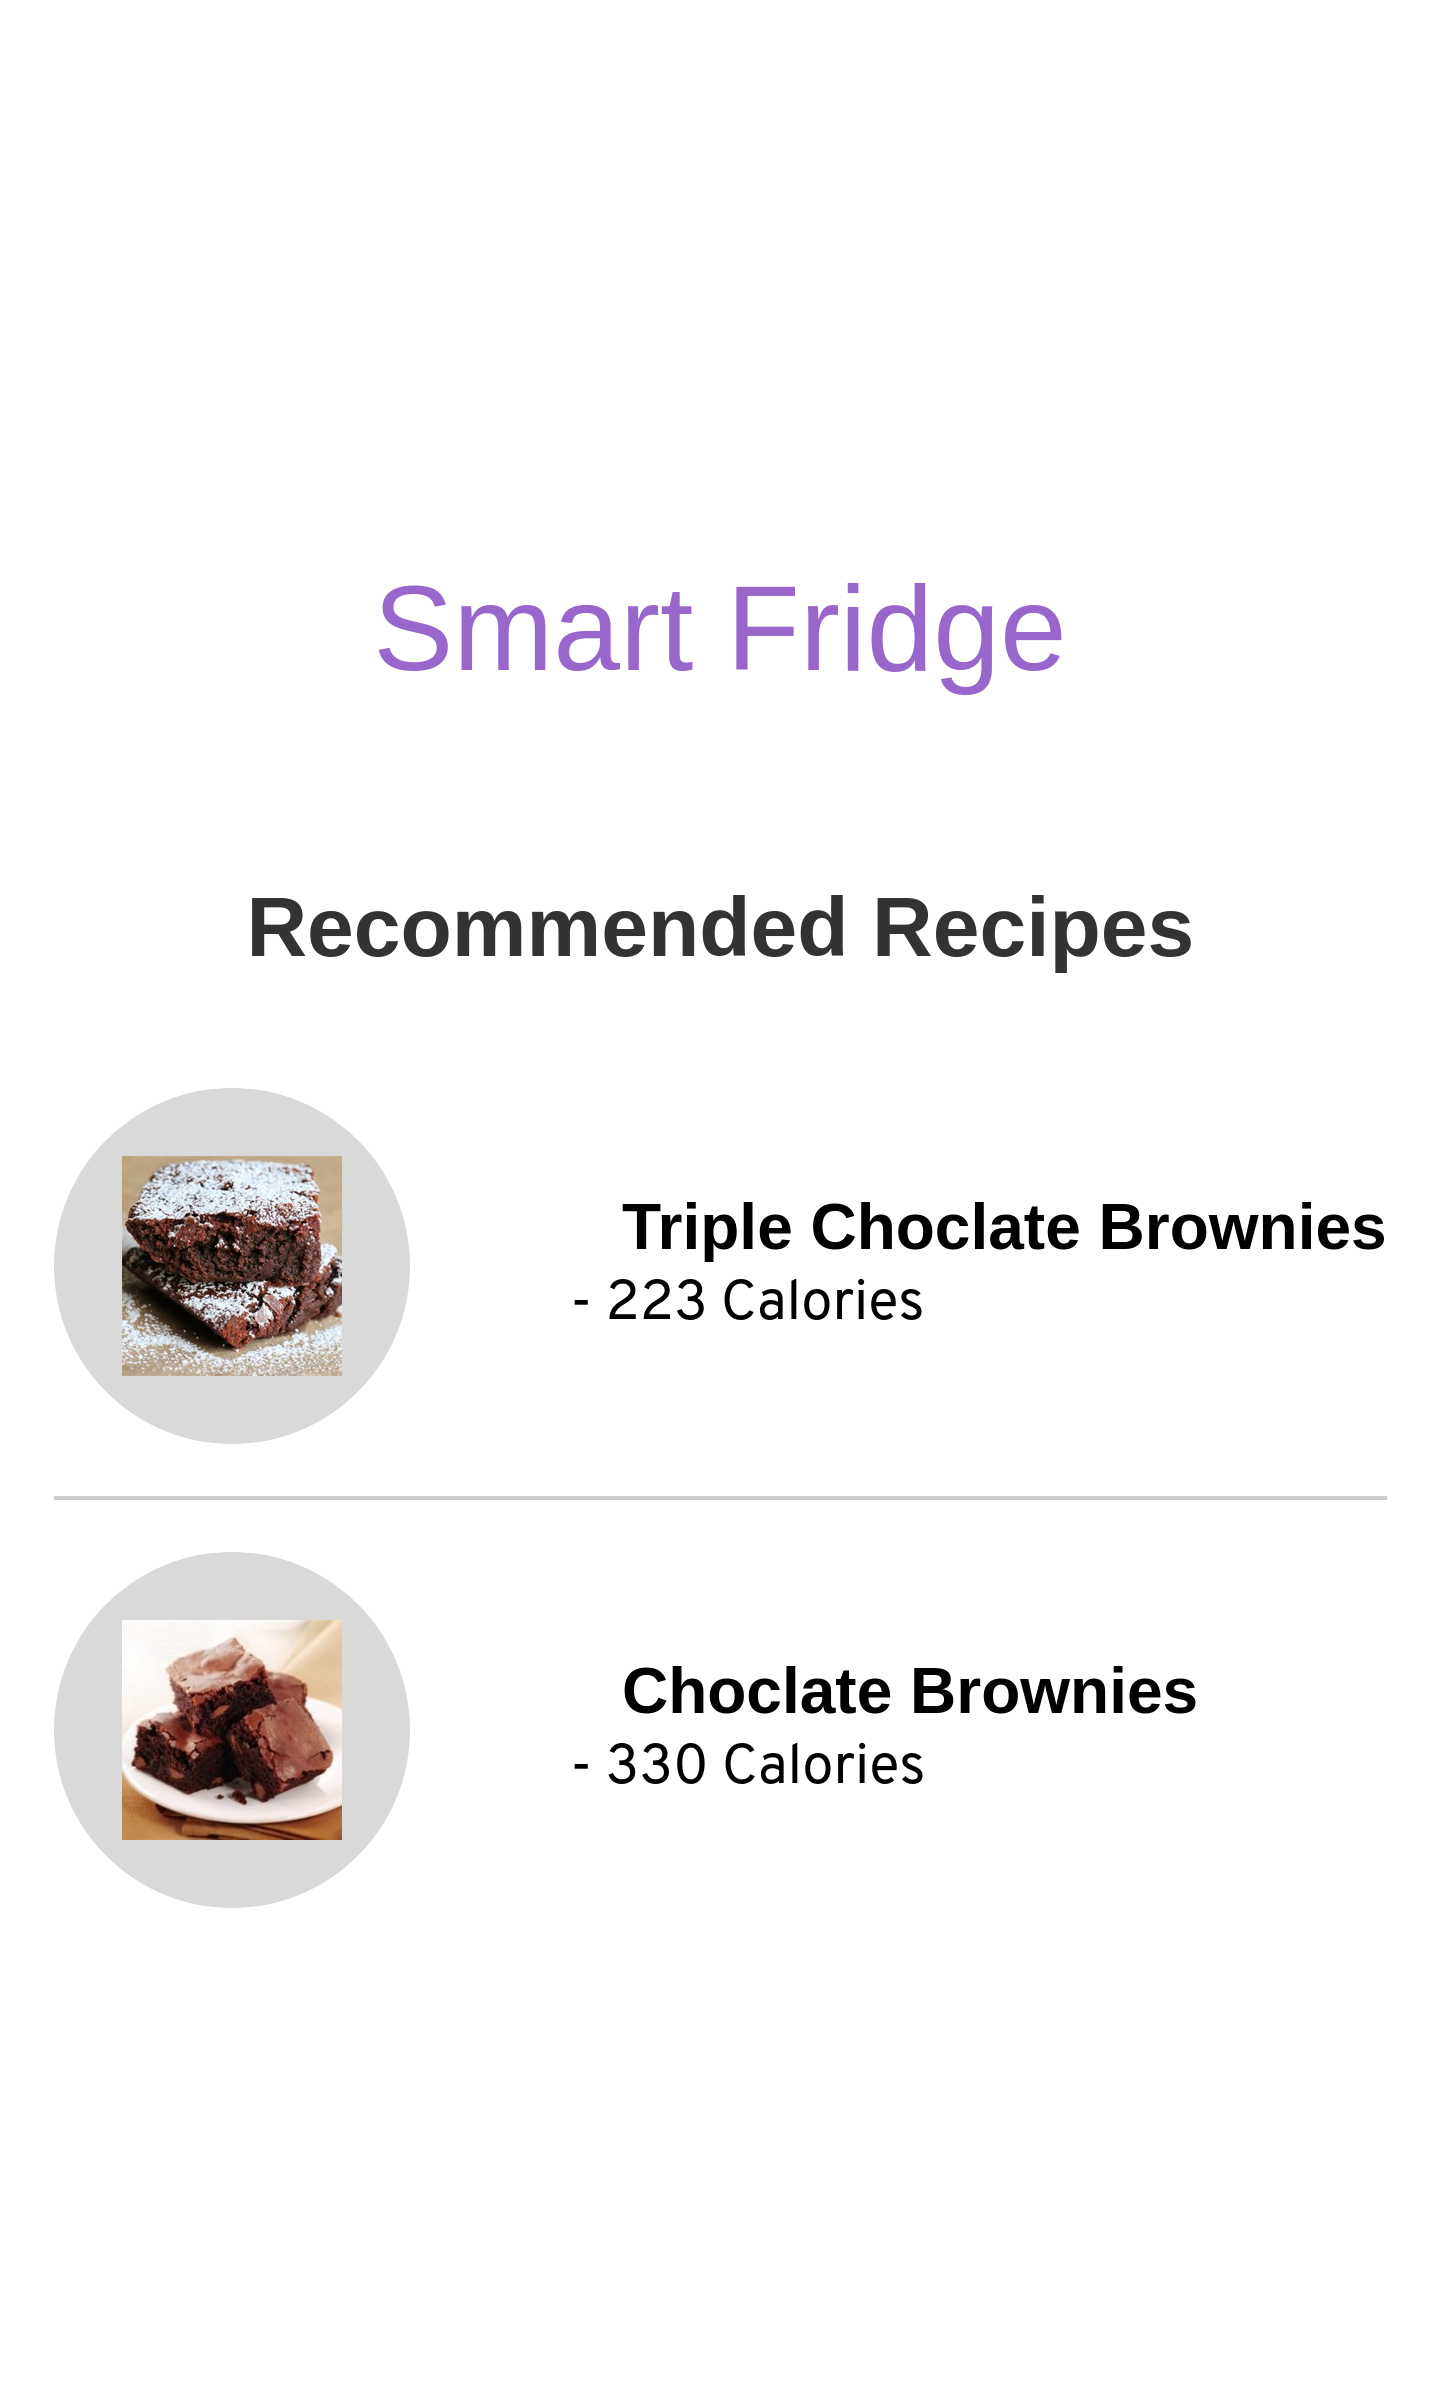
\includegraphics[width=.8\linewidth]{Chapter 4/app_pic/Rec.png}
    \end{subfigure}
    \caption{Screenshots of App.
Left to Right: Login, inventory, Recipes}
    \label{fig:app}
\end{figure}

The left image shows the Login-In screen, pictured filled with our dummy login details, where the user has to enter their username and password to log in and gain access.
This will only have to be done once, as the login will then store unless the user clears their app data.
The middle shows the primary inventory screen, this is the main screen where the user can view the inventory, seeing the name and expiry date of each of their items as well as a little picture provided by us to represent the item.
They can also manage the inventory if need be, by tapping the item to bring up options allowing the user to modify the expiry date or remove the item entirely.
The button below can be used to add an item by name.
The right image contains the recipe screen presenting the recipes from the API to the user, this screen can be reached by swiping right on the inventory and refreshing by pulling down.
To access a website the user simply clicks anywhere on the entry.
As can be seen, by the similar structure of the inventory and recipes stage, the reusable nature of react components was taken full advantage of the make the app quickly and keep the look consistent.

Testing the core functionality of the app was done throughout development, as a “Minimum Viable Product” approach was taken.
Meaning that the app began as a very bare-bone, but fully functional product which only showed the inventory.
By slowing adding to this base, and constantly testing the core feature, we were able to create a more complicated app whose core features had been thoroughly tested by the end of this initial development.
The app could have been improved with more solid test cases, simply to ensure every case was tested consistently.
More features could also be added, perhaps using the camera on the phone as a backup barcode scanner or taking advantage of the API more by passing more data such as user preferences to the API.
However, even without these additions, the results matched all the set-out goals and the app serves as a useful way for the user to view the collected data.

\subsection{Website [HH]}

The website  for the smart fridge was created to serve as a resource for managing the fridge inventory and searching for recipes.
It was built in Python using the Streamlit framework.
The Edamam API was utilised for its extensive database of quality recipes with a thorough nutritional breakdown.

The inventory data is hosted on Supabase, a cloud database service that provides an interface to access and manage data from external applications.
Supabase offers client libraries for several languages, including Python the language of the Smart Fridge website.

\subsubsection{User Login [HH]}

Upon visiting the website, users are prompted to log in or create a new account.
When the correct details are entered, the user can access the main page - the Smart Fridge.
Users remain logged in even after leaving the website thanks to a persistent web cookie.
Passwords are hashed before being stored to protect against unauthorized access.
Users can log out at any time by clicking the "Logout" button in the sidebar.
New accounts can be created by opening an expander.
Session states are used to temporarily store sensitive data that is required while the website is running.


\begin{figure}[H]
    \begin{subfigure}{.5\textwidth}
        \centering
        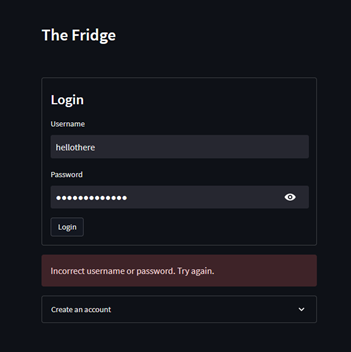
\includegraphics[width=.66\textwidth]{Chapter 4/Hamzah Website/UserLogin/Fig1.png}
        \caption{Demonstration of Login page showing error response}
    \end{subfigure}%
    \begin{subfigure}{.5\textwidth}
        \centering
        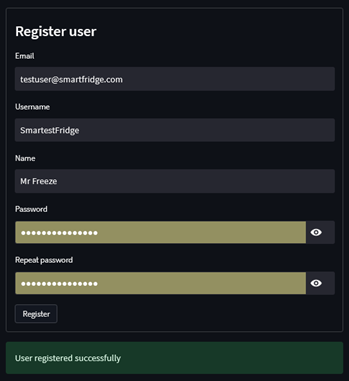
\includegraphics[width=.66\textwidth]{Chapter 4/Hamzah Website/UserLogin/Fig2.png}
        \caption{Registration demonstration}
    \end{subfigure}
    \caption{Login Screens}
\end{figure}

\subsubsection{Home Page [HH]}

The main page displays the user's inventory with useful options below.
The sidebar can be opened by clicking the arrow in the top left corner, where users can log out and access settings.

\begin{figure}[H]
    \begin{subfigure}{.5\textwidth}
        \centering
        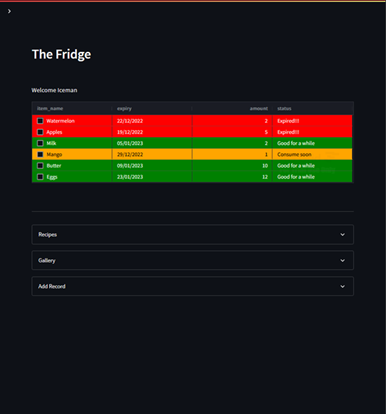
\includegraphics[width=.66\textwidth]{Chapter 4/Hamzah Website/HomePage/Fig3.png}
        \caption{The main page showcasing the inventory}
    \end{subfigure}%
    \begin{subfigure}{.5\textwidth}
        \centering
        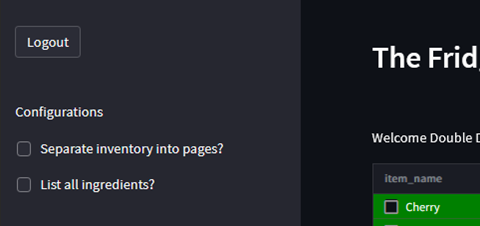
\includegraphics[width=.66\textwidth]{Chapter 4/Hamzah Website/HomePage/Fig4.png}
        \caption{The sidebar options}
    \end{subfigure}
    \caption{Home Page}
\end{figure}

\subsubsection{Fetching Data [HH]}

The website connects to the database using the Supabase client library and authenticates the connection with a URL and key.
SQL statements are used to retrieve and modify data stored in the database.
To retrieve the inventory data, an SQL select statement is used to specify the columns to show to the user, with a condition to only access data that belongs to the current user.

\begin{figure}[H]        
    \centering
    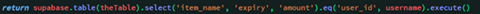
\includegraphics[width=1\textwidth]{Chapter 4/Hamzah Website/FetchingData/Fig5.png}
    \caption{SQL statement to retrieve the fridge inventory from Supabase}
\end{figure} 

\subsubsection{Inventory table [HH]}

To display the inventory, we chose to use a table.
Tables are readable and suited for displaying large data sets.

\begin{figure}[H]        
    \centering
    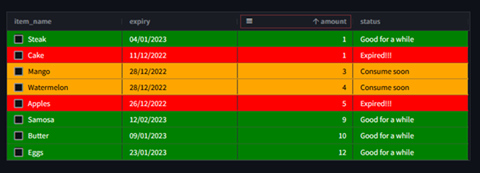
\includegraphics[width=.66\textwidth]{Chapter 4/Hamzah Website/InventoryTable/Fig6.png}
    \caption{Inventory sorted by quantity}
\end{figure} 

The table includes columns for the item name, expiration date, quantity, and status of each item in the inventory.
These columns were chosen because they convey the most relevant and useful information to the user.
Each row is highlighted in a colour corresponding to their expiration status.
Green is for food that is good for a while, orange if only a few days remain until expiration, and red for expired food items that should be handled with caution.

The table can be sorted by clicking on any column, which allows users to easily find specific items or view their inventory in different ways.
For example, they could sort by expiration date to see which items need to be used up first.

In addition to sorting, the table allows users to rearrange columns by dragging them to a new position or hide columns by dragging them outside of the table.
Users can also filter values in a column by clicking on the hamburger icon that appears when hovering over a column.

\begin{figure}[H]        
    \centering
    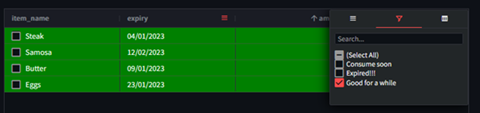
\includegraphics[width=.66\textwidth]{Chapter 4/Hamzah Website/InventoryTable/Fig7.png}
    \caption{Filtering option inside the hamburger menu}
\end{figure} 

An option to paginate the table exists in the sidebar.
Pagination separates rows into different pages to make it easier to navigate.
This is especially useful when the inventory contains a large number of items.

\begin{figure}[H]        
    \centering
    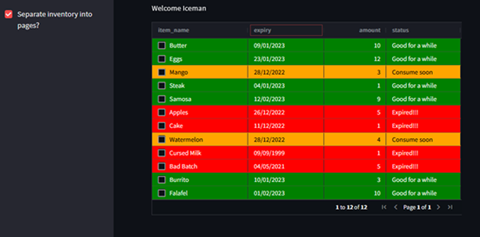
\includegraphics[width=.66\textwidth]{Chapter 4/Hamzah Website/InventoryTable/Fig8.png}
    \caption{Pagination option}
\end{figure} 

The data from Supabase was stored using the Pandas DataFrame and presented using an AgGrid.
The DataFrame is a flexible and mutable two-dimensional table, while the grid was designed to be used in web applications.
The AgGrid JavaScript-based grid type that has useful applications such as allowing us to execute useful commands (such as JavaScript code), but is not as flexible within Python.
Using Pandas alongside the AgGrid grants access to the useful qualities of both.

Since the expiration status is not stored in the database, the website must be able to determine it based on known information.
I created a function which returns the difference in days between an input date and the current day.
The parser function can extract a date from a string containing a date in a many different formats, (such as the different regional date formats like, or different delimiters such as '/' and '-').This is also done for the today date to prevent a ValueError exception that would occur if the expiration date was in a different format to the standard 'datetime' format'.

\begin{figure}[H]        
    \centering
    \includegraphics[width=.66\textwidth]{Chapter 4/Hamzah Website/HowItWasCoded/fig9.png}
    \caption{Function that calculates the difference in days, regardless of format}
\end{figure} 

For each date in the table, the difference in days was calculated and stored in a list.
If the difference in days is negative, then it indicates that the food is already expired.
Otherwise, the food is still safe to eat.
Based on the comparisons shown in \ref{fig:awefulcode}, the specified string of text is stored in a new column of the table, reflecting the status of each item.


\begin{figure}[H]
    \begin{subfigure}{.5\textwidth}
        \centering
        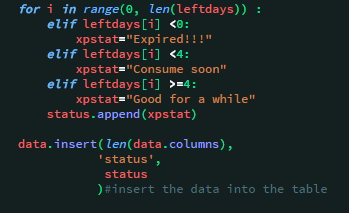
\includegraphics[width=.66\textwidth]{Chapter 4/Hamzah Website/HowItWasCoded/fig10.png}
        \caption{Code that evaluates expiration status and inserts it to the table.}
        \label{fig:awefulcode}
    \end{subfigure}%
    \begin{subfigure}{.5\textwidth}
        \centering
        \includegraphics[width=.66\textwidth]{Chapter 4/Hamzah Website/HowItWasCoded/fig11.png}
        \caption{JavaScript code that changes appearance of a grid based on expiration evaluation, and code that creates and configures the grid.}
        \label{fig:badcode}
    \end{subfigure}
    \caption{Code Snippets}
\end{figure}

The grid configurations are set before it is displayed.

In Fig \ref{fig:badcode} Line 203 to 224 shows the JavaScript code (JsCode) used to modify the colour of the grid.
The status column on the grid will contain one of the three conditional values, and so will be red, orange or green depending on its expiration status.

To execute the JsCode, we must use an AgGrid.
As we transfer the data from the DataFrame to the grid, we also configure the grid to use checkboxes (facilitating record deletion) and allow JsCode.

Line 228 allows the grid to be edited by clicking a cell and typing on a keyboard.
This showcases a potential method to directly edit the values to the database.

\subsubsection{Adding Records [HH]}

To add new items to the inventory, users can enter the name, expiration date, and quantity in the "Add Record" tab.
The expiration date can be chosen from a calendar input widget or entered manually.

\begin{figure}[H]        
    \centering
    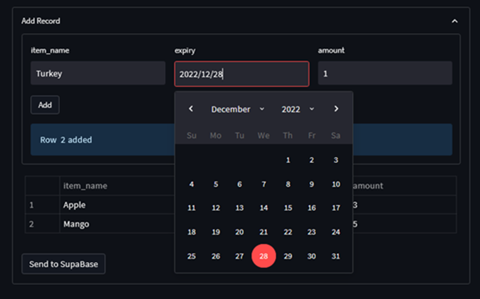
\includegraphics[width=.66\textwidth]{Chapter 4/Hamzah Website/AddingRecords/Fig12.png}
    \caption{Interface to add new items to the database}
\end{figure} 

Calendar widget used for date entry.

When the "Send to SupaBase" button is clicked, the data in the table is converted into a list of dictionaries.
This format allows multiple items to be inserted correctly using an SQL insert statement.
The inventory table is then automatically updated, and the "Add Record" table is reset for adding more items.

Three columns for data input are created, based on the Pandas DataFrame existing in the session state.
An array stores the inputs until the records are submitted.

When new records are sent to the Supabase, they must be assigned a username key, otherwise it will not be recognised to be part of the current user's inventory.
Since the DataFrame already needs to be converted into a list of dictionaries , adding a new key and value is simple.
Now the data can be inserted into the database with the SQL insert statement on line 567.

\begin{figure}[H]
    \begin{subfigure}{.5\textwidth}
        \centering
        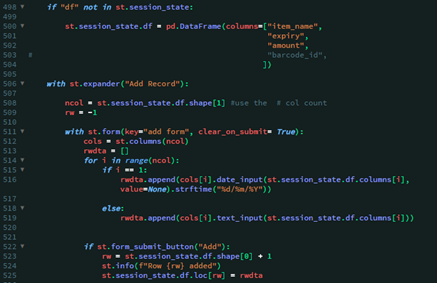
\includegraphics[width=.66\textwidth]{Chapter 4/Hamzah Website/AddingRecords/Fig13.png}
        \caption{Code for creating and accepting data inputs}
    \end{subfigure}%
    \begin{subfigure}{.5\textwidth}
        \centering
        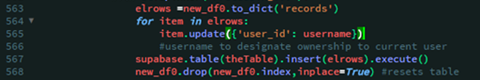
\includegraphics[width=.66\textwidth]{Chapter 4/Hamzah Website/AddingRecords/Fig14.png}
        \caption{Code designated the ownership of new items to the user that added them}
    \end{subfigure}
    \caption{Code Snippets 2}
\end{figure}


\subsubsection{Deleting Records [HH]}

To delete items from the inventory, users can select multiple items using the checkboxes and confirm deletion with a prompt.
The selected items are then removed from the database using an SQL delete statement.



\begin{figure}[H]        
    \centering
    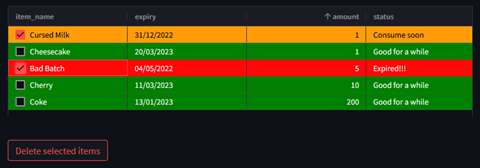
\includegraphics[width=.66\textwidth]{Chapter 4/Hamzah Website/DeletingRecords/Fig15.png}
    \caption{Demonstration of how items are deleted from the table using checkboxes}
\end{figure} 

When the grid was configured, I created a response that returns the values selected by the user.
I programmed the 'Delete' button to appear only if items are selected.
When clicked, the grid is converted into a list, and processed into an SQL statement which deletes item with the matching details.

The 'in' method allows a list to be specified.

\begin{figure}[H]        
    \centering
    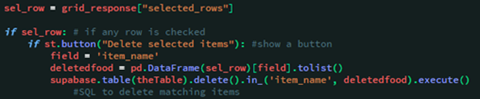
\includegraphics[width=.66\textwidth]{Chapter 4/Hamzah Website/DeletingRecords/Fig16.png}
    \caption{Converting selected items into a suitable format for SQL deletion}
\end{figure} 

\subsubsection{Searching for Recipes [HH]}

Recipes can be found based on items in the fridge.
Recipes can also be filtered based on dietary requirements such as Kosher, low-sugar and vegan, or by the calories per serving.
Drop down menus are used to select the ingredients and dietary requirements.
The nutritional options (calories, carbohydrates and sugar) can be specified by keyboard input or the positive and negative buttons on the box.
The  value can be left at 0 if the user does not wish to specify a requirement.

\begin{figure}[H]
    \begin{subfigure}{.5\textwidth}
        \centering
        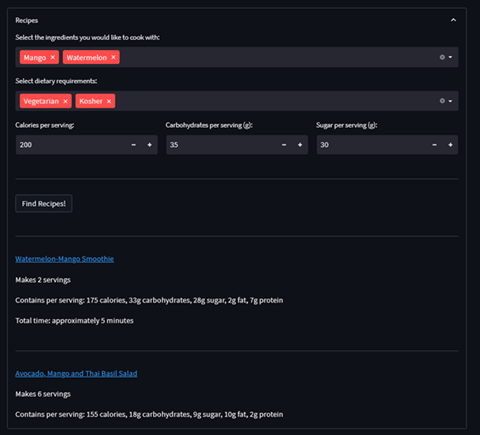
\includegraphics[width=.66\textwidth]{Chapter 4/Hamzah Website/SearchingForRecipes/Fig17.png}
        \caption{Fig demonstrating the recipe interface with generated recipes showing nutritional information}
    \end{subfigure}%
    \begin{subfigure}{.5\textwidth}
        \centering
        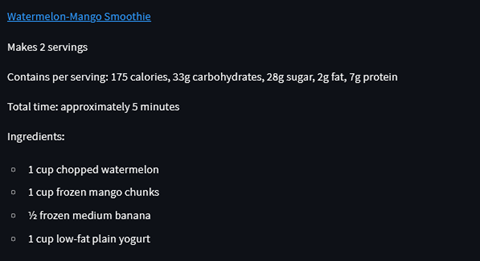
\includegraphics[width=.66\textwidth]{Chapter 4/Hamzah Website/SearchingForRecipes/Fig18.png}
        \caption{Recipes with the ingredients listed}
    \end{subfigure}
    \caption{Recipe Display}
\end{figure}

After the search button has been clicked, the Edamam API returns the available recipes.
If there are no available recipes, then the website will prompt the user to reconsider the search parameters.

For each recipe, a link to the original website is displayed, along with additional data such as nutritional information based on servings, preparation time, and the ingredients needed for the recipe.
For a more compact view, the recipe list can be disabled from the sidebar.

A URL is used to interact with the Edamam API.
It is composed of an application ID and key (received when signing up), ingredients, and optional parameters such as dietary requirements.

\begin{figure}[H]        
    \centering
    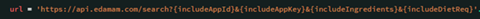
\includegraphics[width=.66\textwidth]{Chapter 4/Hamzah Website/SearchingForRecipes/Fig19.png}
    \caption{the URL format accepted by Edamam API}
\end{figure} 

When the user selects their choice of ingredients and dietary requirements, they are stored in a list.

Ingredients and dietary requirements are formatted slightly differently in the Edamam URL.
In both cases, the 'join' function concatenates each element of the list with the string specified in inverted commas.

The API returns recipe data in the JSON format which is convenient to parse.
At this point, the recipes are evaluated against the nutritional conditions set by the user.
The recipes that meet the criteria, they are displayed with the aforementioned information.

\begin{figure}[H]
    \begin{subfigure}{.5\textwidth}
        \centering
        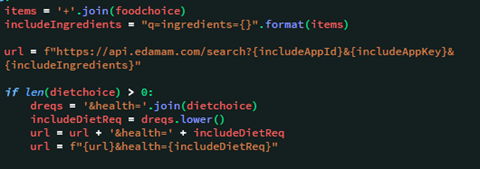
\includegraphics[width=.66\textwidth]{Chapter 4/Hamzah Website/SearchingForRecipes/Fig20.png}
        \caption{Code showing how the user choices are formatted into an Edamam query.}
    \end{subfigure}%
    \begin{subfigure}{.5\textwidth}
        \centering
        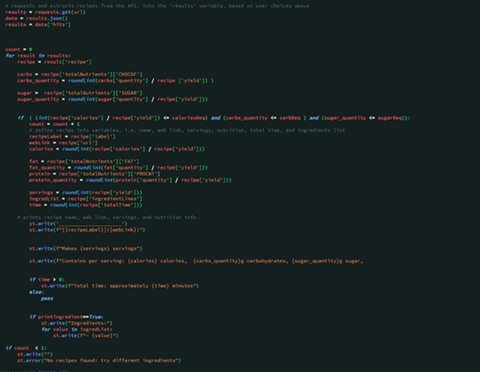
\includegraphics[width=.66\textwidth]{Chapter 4/Hamzah Website/SearchingForRecipes/Fig21.png}
        \caption{Code showing how the JSON data received by Edamam API is processed and displayed to the user.}
    \end{subfigure}
    \caption{Code Snippets 3}
\end{figure}

\subsubsection{Developments [HH]}

My first prototype started with reading a CSV file and displaying them on the screen.
The aim of this was to demonstrate how data could be displayed.
The CSV file was read and parsed into a DataFrame.
It was imperative to use a cloud-hosted database solution, so the website soon transitioned over.

When I first used the Supabase library to insert the items, the result were less than ideal: the items were added as a 'dictionary' and were all contained in one cell.

I then switched to another SQL module in python, known as Psycopg2.
I was able to insert items correctly.
I extracted the values from the Dataframe, concatenated them into a single string and then inserted them into the database.
Psycopg2 uses a 'server cursor' which is an “object that enables traversal over the rows of a result set”.

While it was an effective solution, there was a caveat.
An additional database password would have to be created and stored somewhere; without a password Psycopg2 is unable to connect.
This is not inherently a big issue, but since we executed other SQL statements with the Supabase client library, it made sense to use it where possible.

By examining the Pandas documentation \cite{pd}, I discovered some useful data manipulation functions.
The DataFrame could be converted into a dictionary using the function 'pandas.DataFrame.to\_dict('records)'.
If multiple items exist in the DataFrame it is converted into a list of dictionaries.
 In the list, each dictionary represents a single record.
The keys in the dictionaries corresponds to the column names in the database, and the values represent the data to be inserted for each column.
This method worked perfectly with the Supabase library.
Inserting the items this way ensured that each item and their respective details were contained in the correct place.